\documentclass[11pt,letterpaper]{article}
\usepackage{geometry}
\geometry{margin=1in}
\usepackage{graphicx}
\usepackage{subcaption} %for subfigures
\usepackage{float}

\setlength{\parindent}{0pt}
\setlength{\parskip}{0.5em}

%make lists tighter
\usepackage{enumitem}
\setlist{nolistsep}

%reduce spacing before and after section
\usepackage{titlesec}
% reduce section, subsection, etc spacing
\usepackage{titlesec}
\titlespacing*{\section}{0pt}{0\baselineskip}{0\baselineskip}
\titlespacing*{\subsection}{0pt}{0\baselineskip}{0\baselineskip}
\titlespacing*{\subsubsection}{0pt}{0\baselineskip}{0\baselineskip}

%reduce list spacing
\usepackage{enumitem}
\setlist{nosep}

\usepackage[style=apa]{biblatex}
\addbibresource{../other/references.bib}

\usepackage[hidelinks]{hyperref}

\title{Lab 4 - Cloud Data, Stat 215A, Fall 2024\vspace{-2em}}

% submission must not contain any of your names
% but feel free to make a version for yourself with your names on it
% \author{Your names}

\begin{document}
\maketitle

\section{Introduction}
Global climate change has been a huge concern over the past few decades. As the amount of carbon dioxide and greenhouse gases increase in the atmosphere, more heat is trapped, resulting in global warming. It is well known that carbon dioxide is responsible for about 70\% of global warming. Compared to the rest of the globe, the Arctic suffers much more from climate change. According to Rantanen et al., arctic warming is four times faster than the globe on average \parencite{rantanen2022arctic}. The cascading impacts of global warming threaten many facets of the Arctic, such as decreasing biodiversity (marine species) and accelerated shoreline erosions. More importantly, global warming causes ice to melt in the Arctic, speeding up the rise in temperature even more as water absorbs sunlight, and ice reflects it.

As the Arctic continues to warm over the next few years, it is possible that the distribution of clouds in the arctic will change too. Clouds are important as they impact the energy flow in the Arctic climate system by modulating radiative and non-radiative energy, affecting surface/atmospheric temperature and arctic circulation \parencite{taylor2023isolating}. Thus, it is important for us to study the distribution of arctic clouds and their changes in response to climate change. However, the domain problem for this lab is that clouds are hard to study or detect because cloud particles with ice and water have similar properties to particles on ice- and snow- surfaces \parencite{shi2008daytime}. The goal of our lab is to build an algorithm for cloud detection that can distinguish a cloud from a non-cloud.

In this lab, we first performed some exploratory analysis on the three given images to see if there is any feature that is a good predictor for cloud detection. Then auto-encoder was used as a feature engineering tool to encode the data into a lower dimensional space and reconstruct the images. After splitting the data, we performed logistic regression, random forest, weighted ensemble, and neural network and determined the best classification model for cloud detection.


\section{Data}
\label{sec:Data}
To tackle the problem of cloud detection in the Arctic, this work uses data collected by the Multi-angle Imaging SpectroRadiometer (MISR) aboard the National Aeronautics and Space Administration's (NASA) Terra satellite. The provided dataset consists of three images, each containing radiance data from the MISR sensor at different angles along with the domain-specific features Normalized Difference Angular Index (NDAI), Standard Deviation (SD), and Correlation (CORR). Moreover, expert labels are provided for each pixel in the images, indicating whether the pixel represents a cloud, non-cloud, or unlabeled due to being in an ambiguous region.

In total, there are 345,556 pixels in all three images, with 60.2 \% of the pixels having expert labels. As depicted in Figure \ref{fig_eda_label_distrib}, 36.8 \% of the labeled pixels are clouds, while 23.4 \% are non-clouds. The remaining 39.8 \% of the pixels are unlabeled due to ambiguity.
\begin{figure}[H]
    \centering
    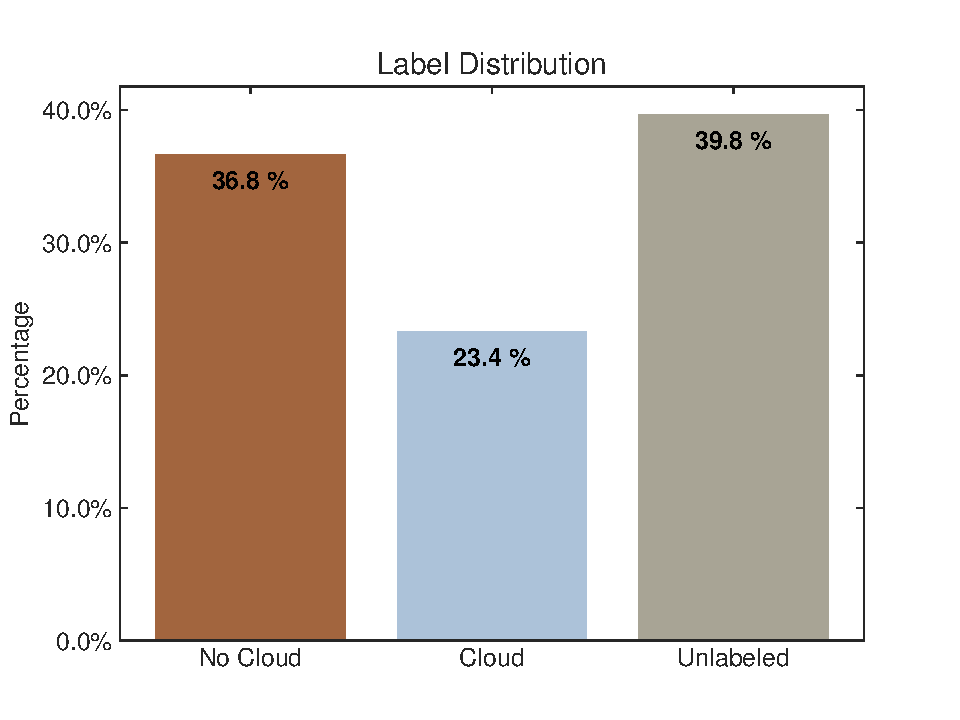
\includegraphics[width=0.7\linewidth]{figs/eda_label_distribution.pdf}
    \caption{Distribution of expert labels in the provided dataset.}
    \label{fig_eda_label_distrib}
\end{figure}

Figure \ref{fig_eda_label_distrib} shows the spatial distribution of cloud and non-cloud pixels in the images. The figure reveals that unlabeled regions constitute the transition zones between cloud and non-cloud regions, indicating that these areas are challenging to classify.
\begin{figure}[H]
    \centering
    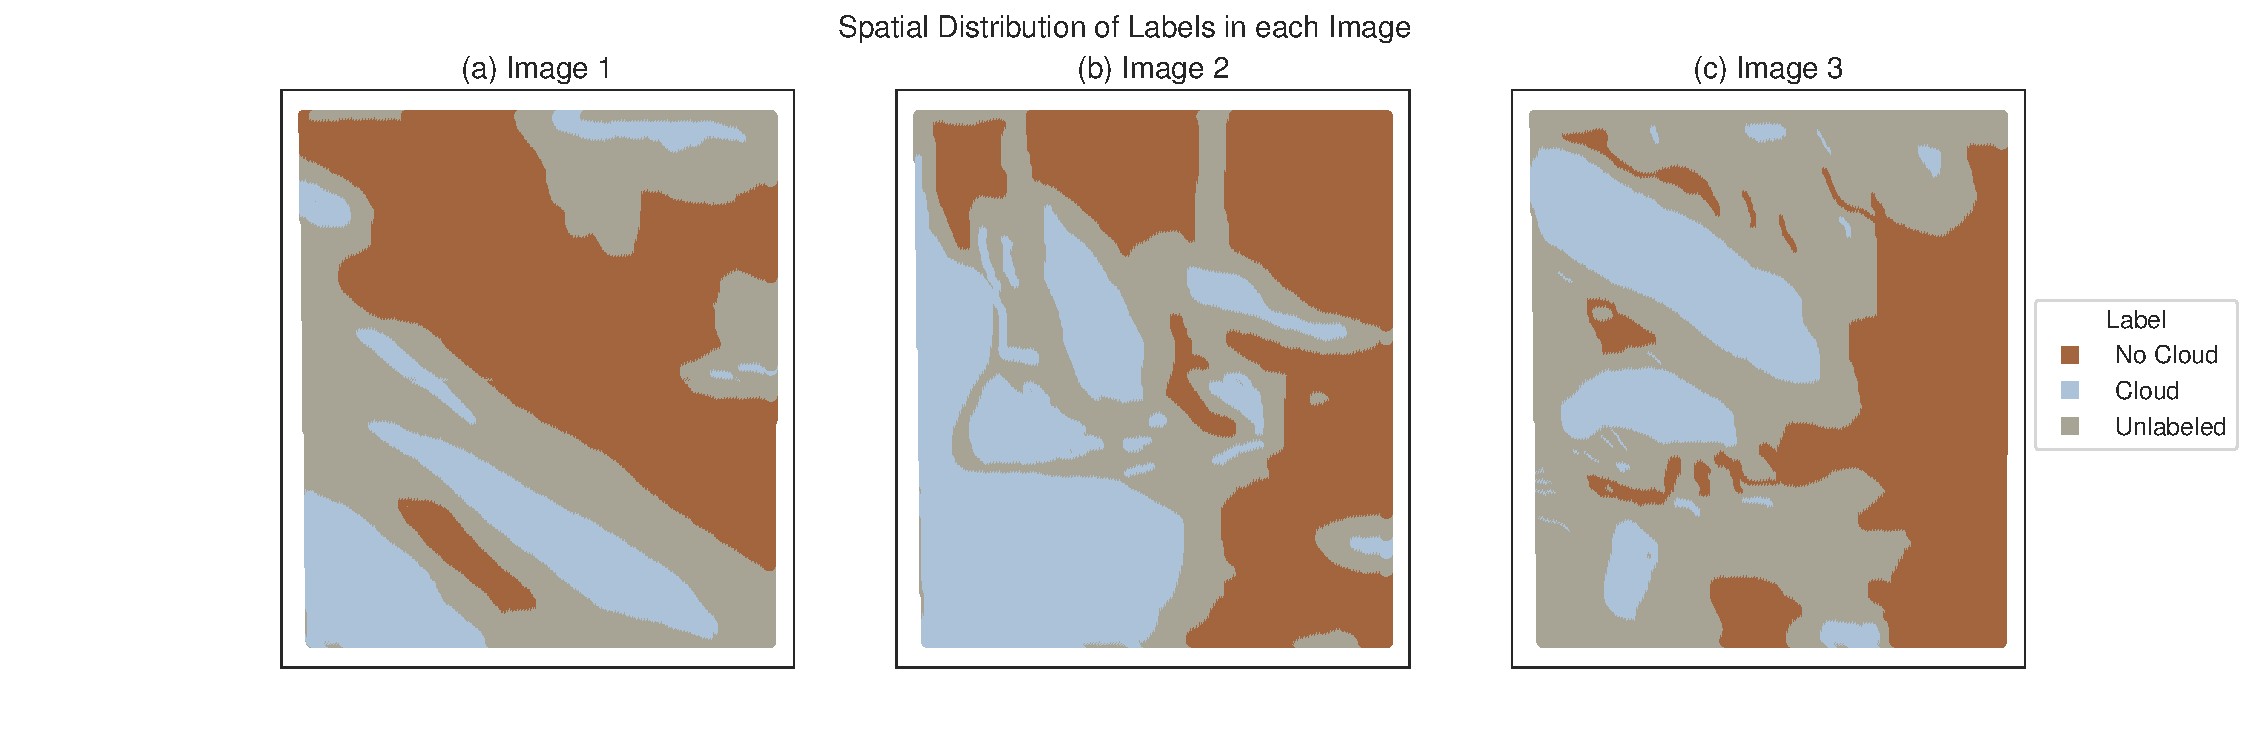
\includegraphics[width=\linewidth]{figs/eda_label_distribution_map.pdf}
    \caption{Spatial distribution of labels for each of the provided images.}
    \label{fig_eda_spatial_distrib}
\end{figure}

To assess whether the provided features can accurately model the presence of clouds, Figure \ref{fig_eda_feature_distrib} displays a violin plot for each feature, comparing the distribution of values for cloud and non-cloud pixels. The plot shows that the features exhibit different distributions for cloud and non-cloud pixels, suggesting that they may be useful for distinguishing between the two classes. Most notably, Figure \ref{fig_eda_feature_distrib}a reveals that the NDAI feature exhibits the most significant difference in distribution between cloud and
non-cloud pixels, indicating its potential importance for cloud detection. Furthermore, the figure suggests that SD (Figure \ref{fig_eda_feature_distrib}b) and CORR (Figure \ref{fig_eda_feature_distrib}c) may be useful as well, as the first quartile of the distributions for cloud pixels is larger than the third quartile for non-cloud pixels. The distributions of the radiance angles (DF, CF, BF, AF, AN – Figures \ref{fig_eda_feature_distrib}d-h) do not show as clear a distinction between cloud and non-cloud pixels, indicating that one of the radiance angles alone is not a good predictor for cloud detection.
\begin{figure}[H]
    \centering
    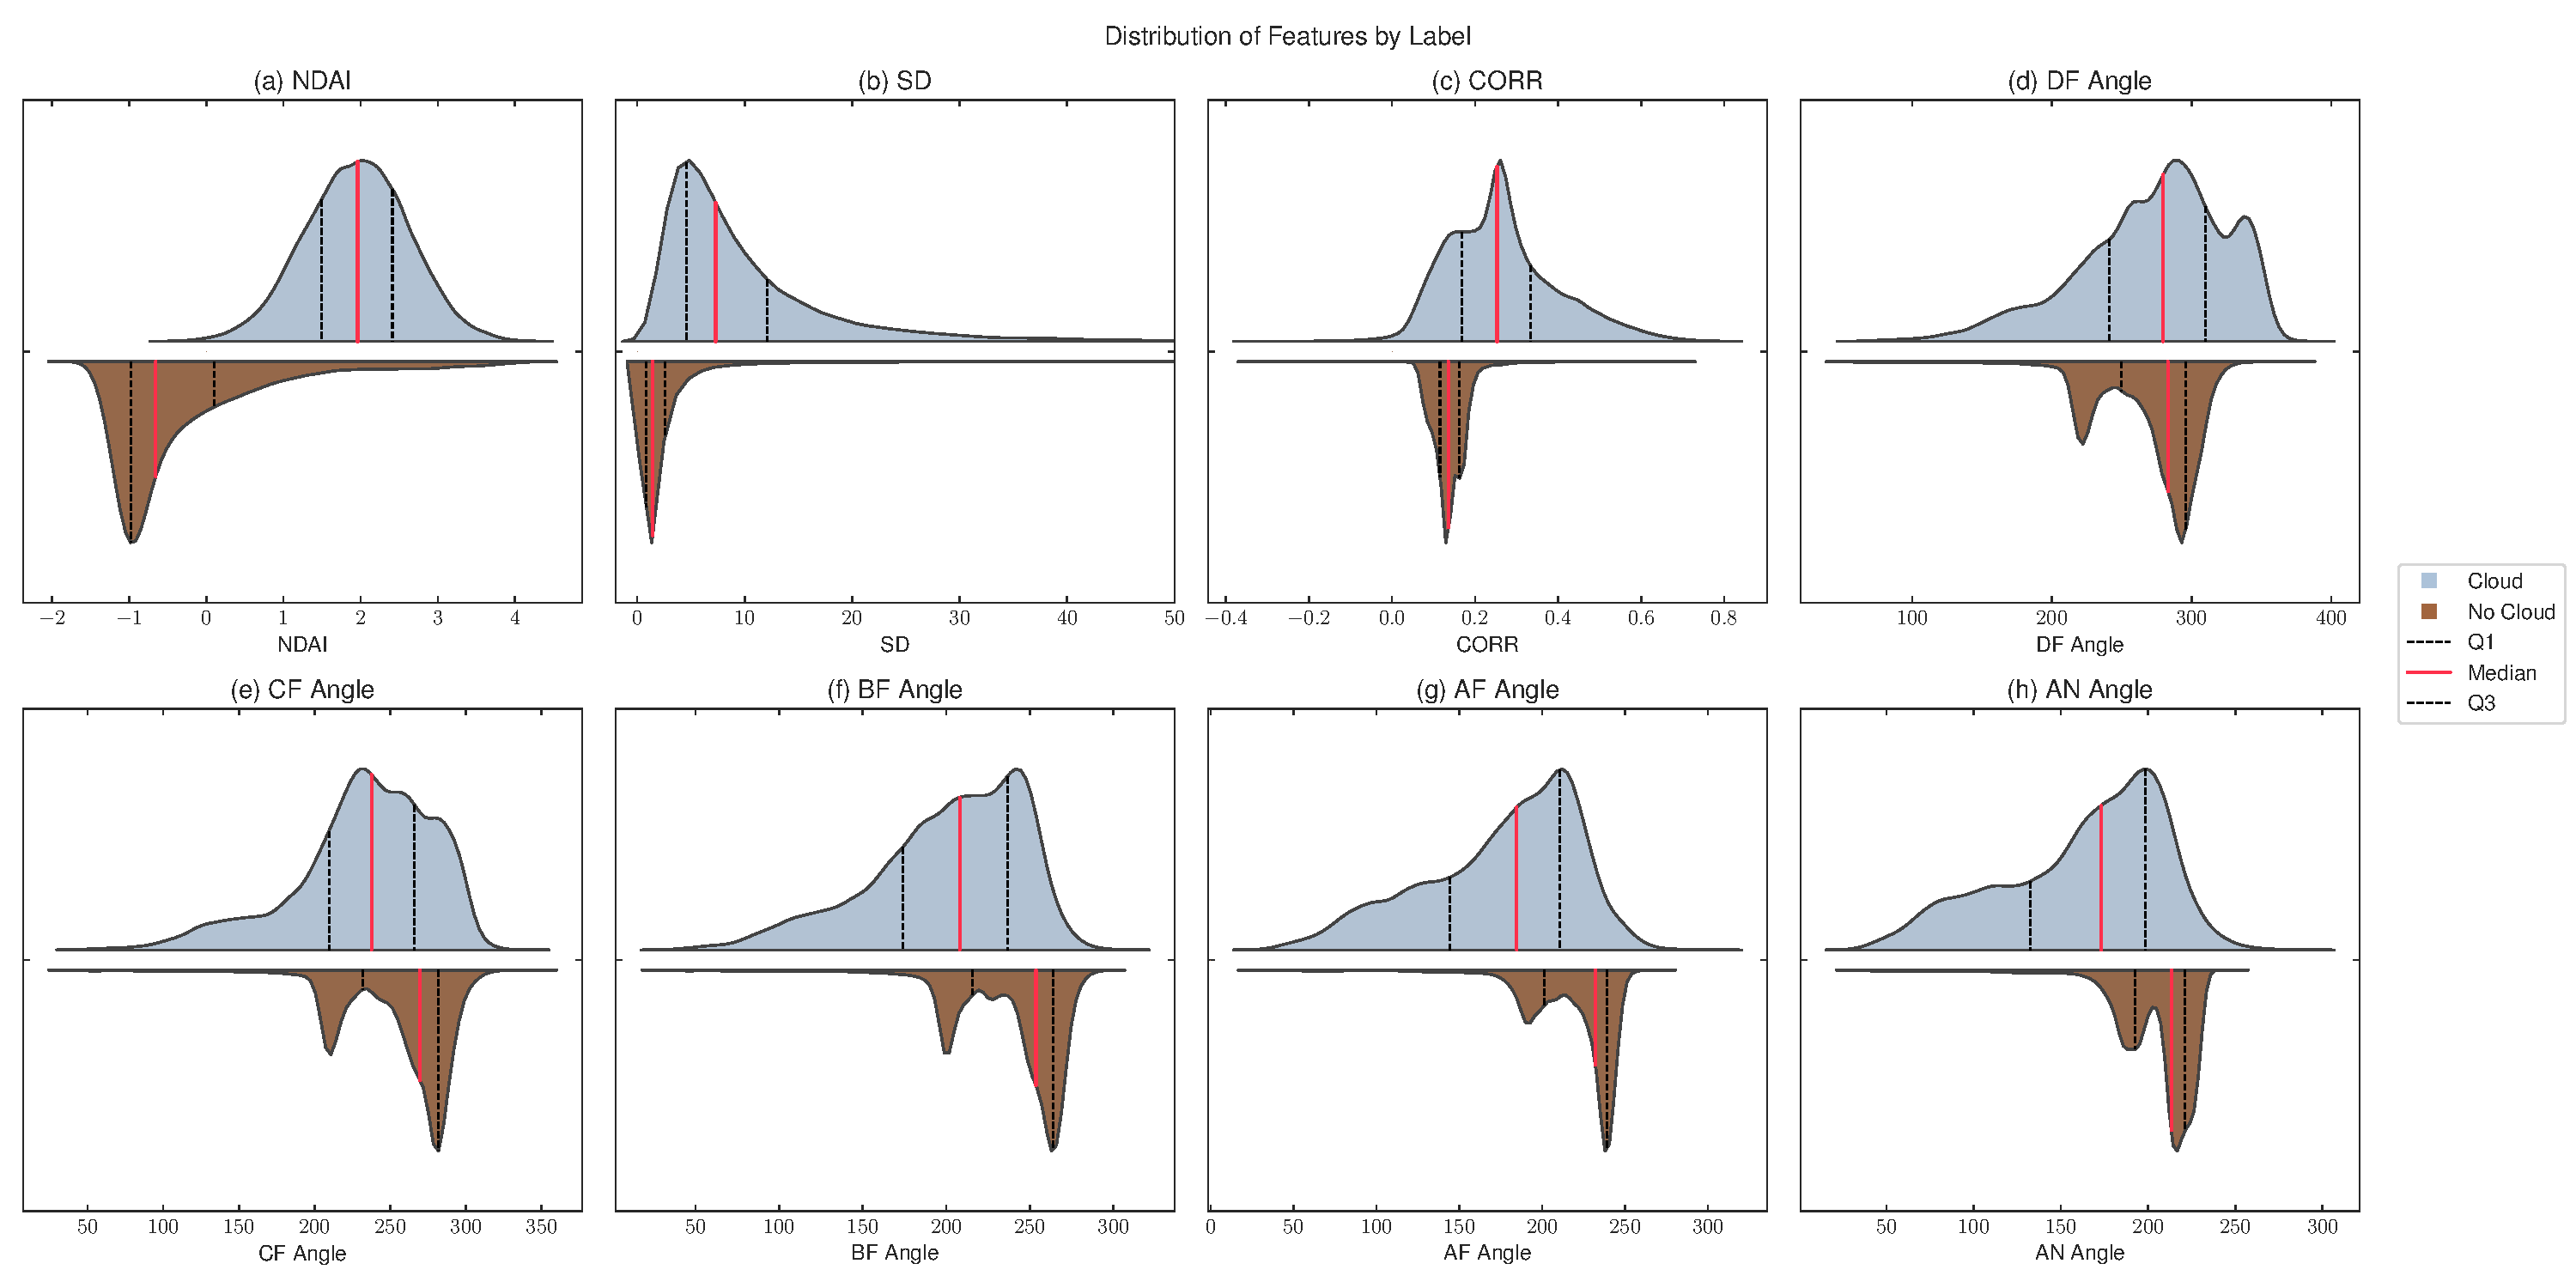
\includegraphics[width=\linewidth]{figs/eda_feature_distribution.pdf}
    \caption{Distribution of features by cloud and non-cloud region.}
    \label{fig_eda_feature_distrib}
\end{figure}

Motivated by these observations, Figure \ref{fig_eda_3d_scatter} shows a 3D-scatter plot of the NDAI, SD, and CORR features, colored by the expert labels. The plot illustrates different clusters of cloud and non-cloud pixels in the feature space, indicating that the features may be effective in distinguishing between the two classes. However, the figure also suggests that the classes are not perfectly separable by a linear hyperplane, underscoring the potential need for non-linear classifiers to model the data effectively.

\begin{figure}[H]
    \centering
    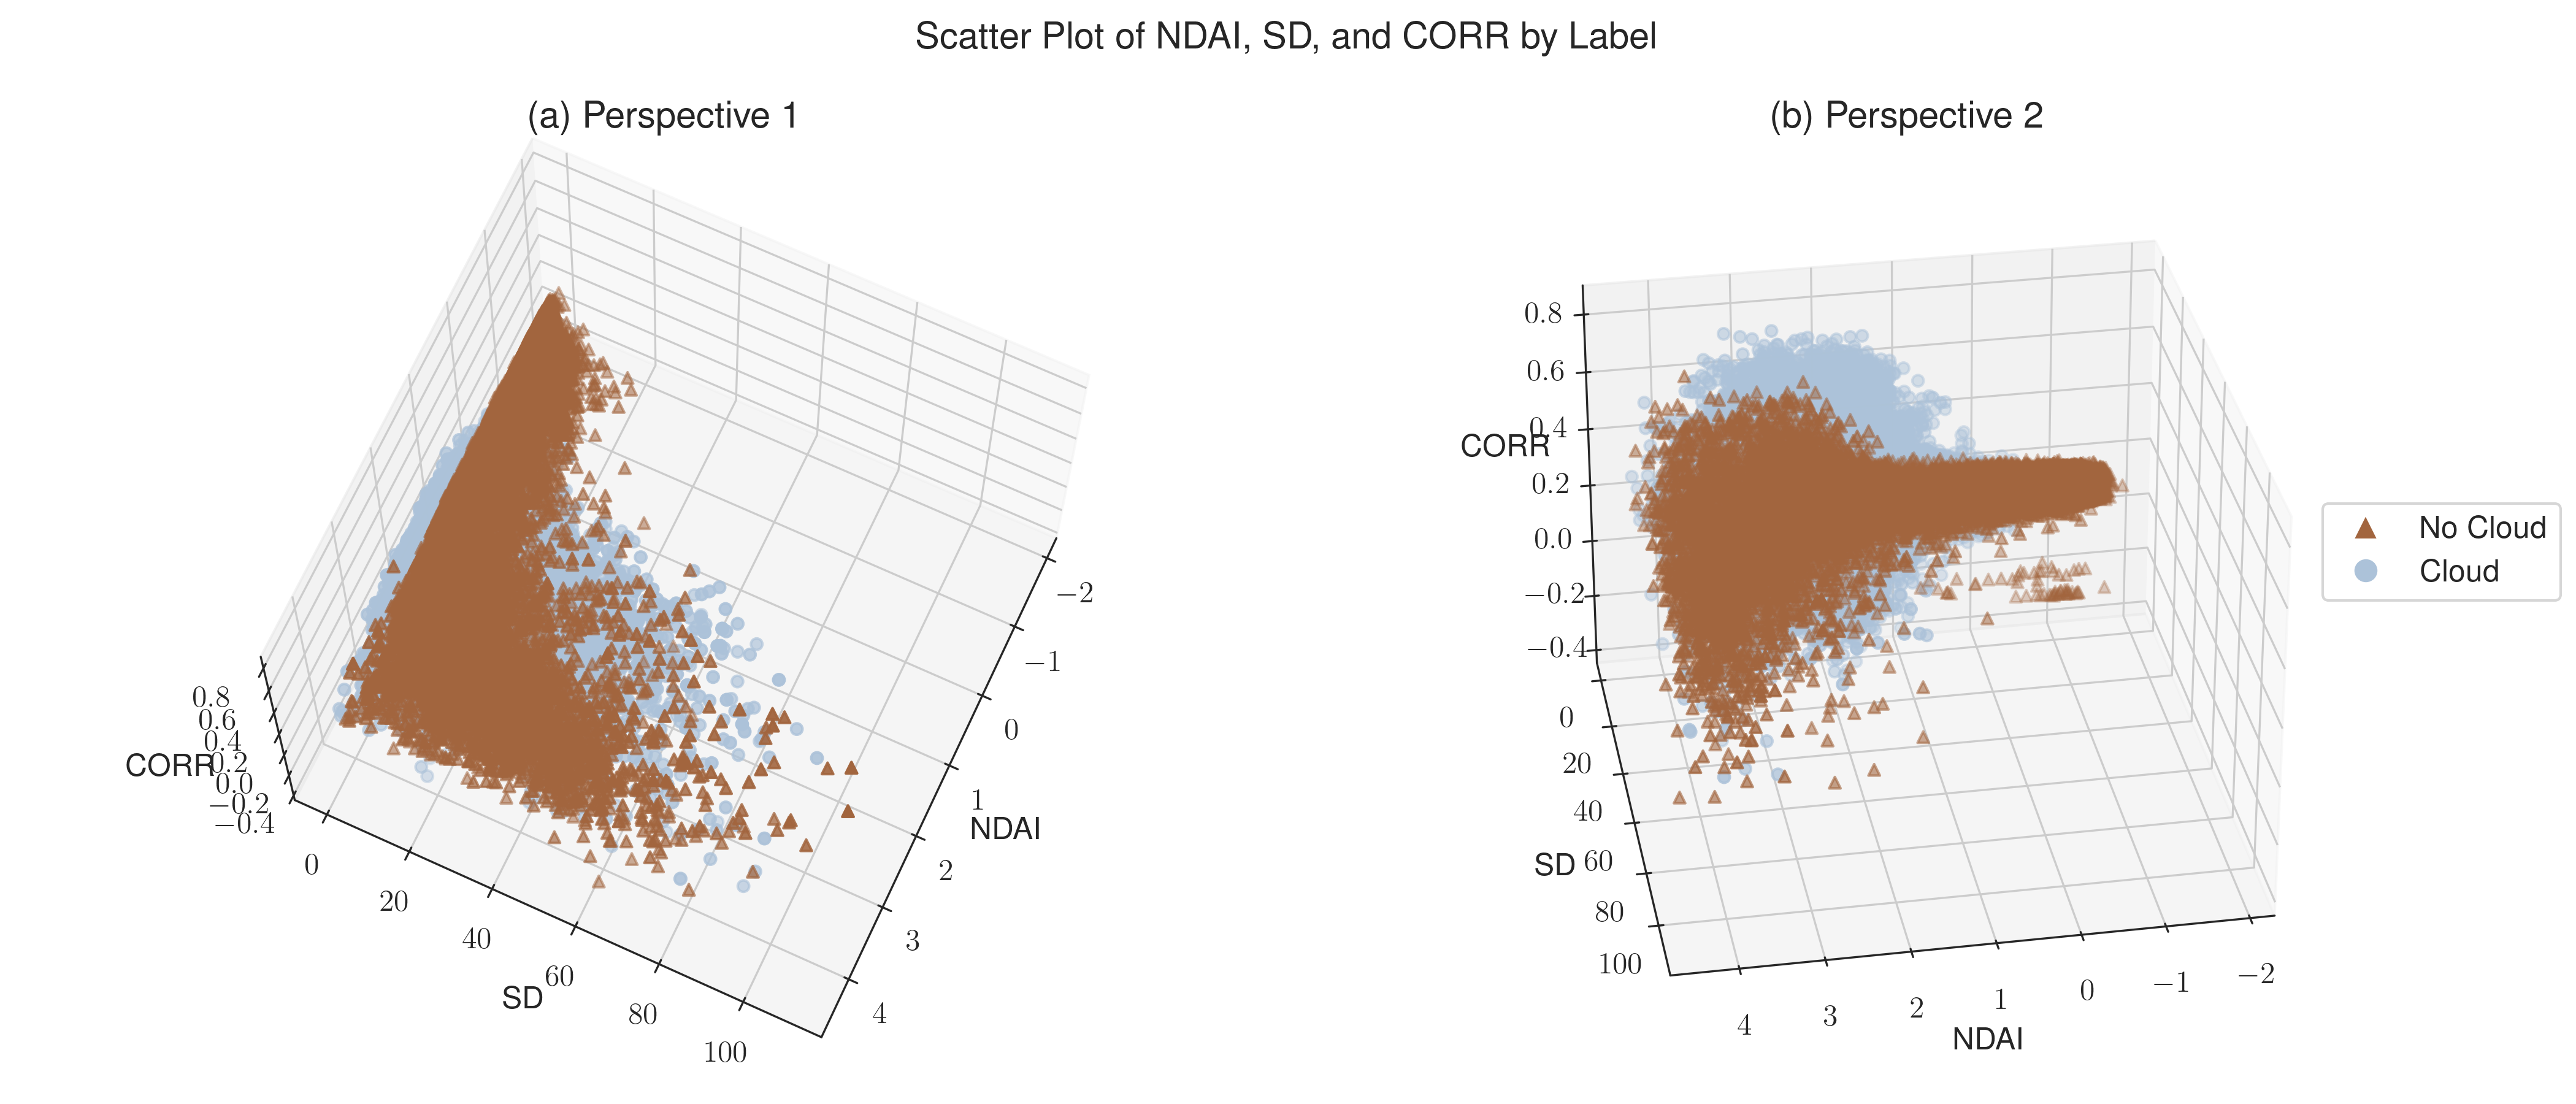
\includegraphics[width=\linewidth]{figs/eda_3d_scatter.png}
    \caption{Scatter plot of NDAI, SD, and CORR features for cloud and non-cloud pixels.}
    \label{fig_eda_3d_scatter}
\end{figure}


\section{Feature selection and engineering}
\label{sec:feature_selection}
Section \ref{sec:Data} explores the data visually and concludes that NDAI, SD, and CORR might be good predictors for the existence of clouds in a MISR image. This section aims to validate these observations by quantifying the relationship between each feature and the cloud presence label using correlation analysis. Furthermore, this section explores the potential of feature engineering by training an Auto-encoder to extract latent representations of the data that may better separate cloud pixels from non-cloud pixels.

To quantify the relationship between the features and the cloud presence label, the point-biserial correlation coefficient is applied. This correlation coefficient measures the strength and direction of the association between continuous variables (the features ) and a binary variable (cloud presence label). Figure \ref{fig_correlation_features} shows a bar plot of the correlation coefficients for each feature. The plot reveals that NDAI, with a correlation coefficient of 0.76, has the strongest relationship with the cloud presence label, followed by CORR (0.55) and the AN radiance angle (–0.5). The SD feature has a slightly weaker correlation coefficient of 0.44. Moreover, it can be concluded that the DF Angle does not correlate at all with the cloud presence label, as its correlation coefficient is close to zero. These results confirm the visual observations from Section \ref{sec:Data} and suggest that NDAI is the most important feature for predicting cloud presence, followed by CORR and AN radiance angle.

\begin{figure}[H]
    \centering
    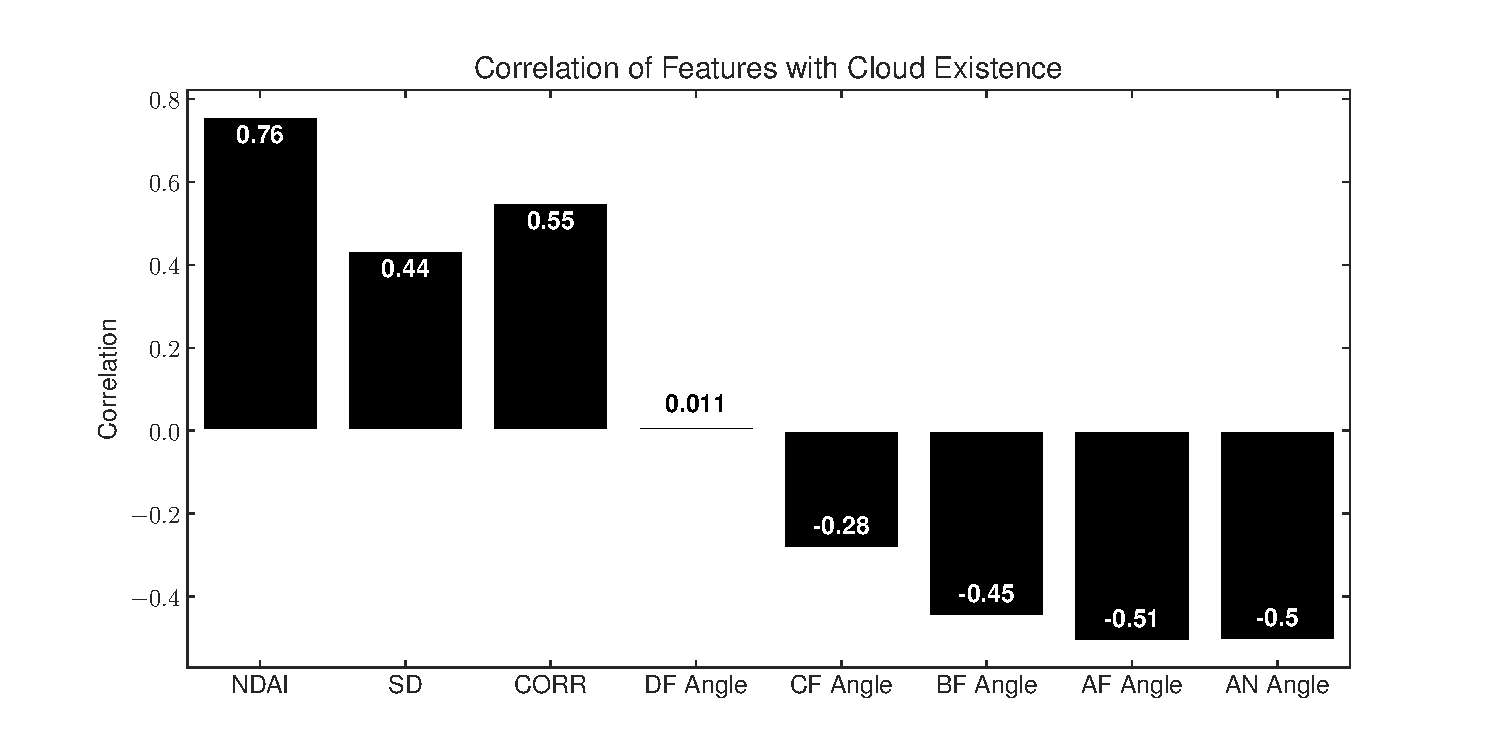
\includegraphics[width=\linewidth]{figs/correlation_features.pdf}
    \caption{Point-biserial correlation coefficients of features with cloud existence labels.}
    \label{fig_correlation_features}
\end{figure}

To assess whether better features can be obtained by learning a latent representation of the images, an Auto-encoder is trained using the PyTorch Lightning library \parencite[]{pytorch_lightning}. The model architecture consists of four down-sampling convolutional layers and four up-sampling convolutional layers, each followed by the rectified linear unit (ReLU) function. The hyper-parameter search for the Auto-encoder is conducted using the Weights and Biases library, leveraging its sweep functionality to efficiently explore the search space \parencite[]{wandb}. Table \ref{table:Auto-encoder_hp_space} outlines the search space, which includes variations in kernel size, embedding size, and the choice of the loss function. The kernel size controls the area of input data processed by each convolution, affecting the extent to which surrounding pixels contribute to the value of the current pixel. The embedding size determines the dimensionality of the latent space, determining how much detail the model can capture and represent in the latent space. To calculate the loss, which is used to update the model weights, two different loss functions are applied: root mean squared error (RMSE) and mean absolute error (MAE). These loss functions are mainly used because they operate on comparable scales, facilitating a consistent evaluation across different hyper-parameter configurations.
\begin{table}[]
\centering
\begin{tabular}{|l|l|}
\hline
\textbf{Hyper-parameter} & \textbf{Values} \\ \hline
Loss                    & RMSE, MAE       \\
Kernel Size             & 3, 5, 7         \\
Embedding Size          & 2, 4, 6, 8      \\ \hline
\end{tabular}
\caption{Hyper-parameter search space for the Auto-encoder.}
\label{table:Auto-encoder_hp_space}
\end{table}

The training process involves using image 1 as the training dataset and image 2 for validation. The goal is to minimize the validation loss, thereby ensuring the model's ability to generalize to unseen data. We also apply early stopping to prevent overfitting. The training loop is suspended if the validation loss does not improve for 10 consecutive epochs, with a maximum limit of 100 epochs. The early stopping mechanism helps maintain a balance between training efficiency and model performance, reducing the risk of overfitting while preventing unnecessarily prolonged training runs.

Table \ref{table:Auto-encoder_best_hp} presents the best hyper-parameters obtained from the search, which result in a validation loss of 12.5846. The training and validation loss curves for this model, shown in Figure \ref{fig_autoencoder_loss}, demonstrate consistent convergence, with no signs of overfitting. This stability indicates that the model successfully learns to encode the features without memorizing the training data.

\begin{table}[]
\centering
\begin{tabular}{|l|l|}
\hline
\textbf{Hyper-parameter} & \textbf{Value} \\ \hline
Loss                    & RMSE            \\ \hline
Kernel Size             & 3               \\ \hline
Embedding Size          & 2               \\ \hline
\end{tabular}
\caption{Hyper-parameters for best Auto-encoder that minimizes the validation loss.}
\label{table:Auto-encoder_best_hp}
\end{table}

\begin{figure}[H]
    \centering
    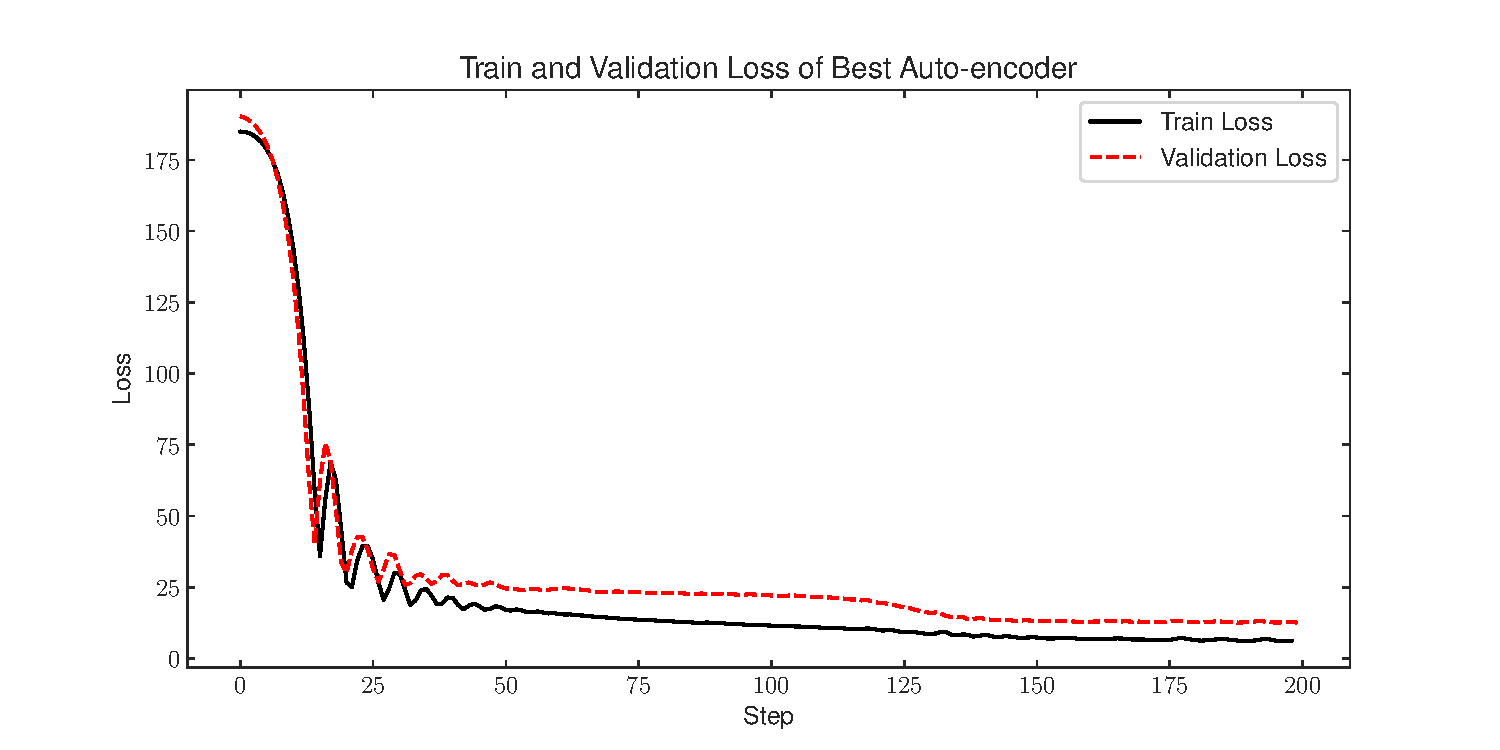
\includegraphics[width=\linewidth]{figs/autoencoder_loss.pdf}
    \caption{Train and validation loss curves of the auto-encoder that minimizes the validation loss.}
    \label{fig_autoencoder_loss}
\end{figure}

The best model from the hyper-parameter search produces 2-dimensional embeddings, allowing for visual inspection of the latent space. Figure \ref{fig_embeddings} shows a scatter plot of these embeddings, with each point colored according to the expert labels for cloud and non-cloud pixels. While some degree of clustering is observable, the separation between cloud and non-cloud pixels is not as clear as when using the original NDAI, SD, and CORR features. This suggests that, despite the Auto-encoder's capacity to learn complex patterns, the domain-specific features provide better discriminative power for distinguishing between cloud and non-cloud pixels.

\begin{figure}[H]
    \centering
    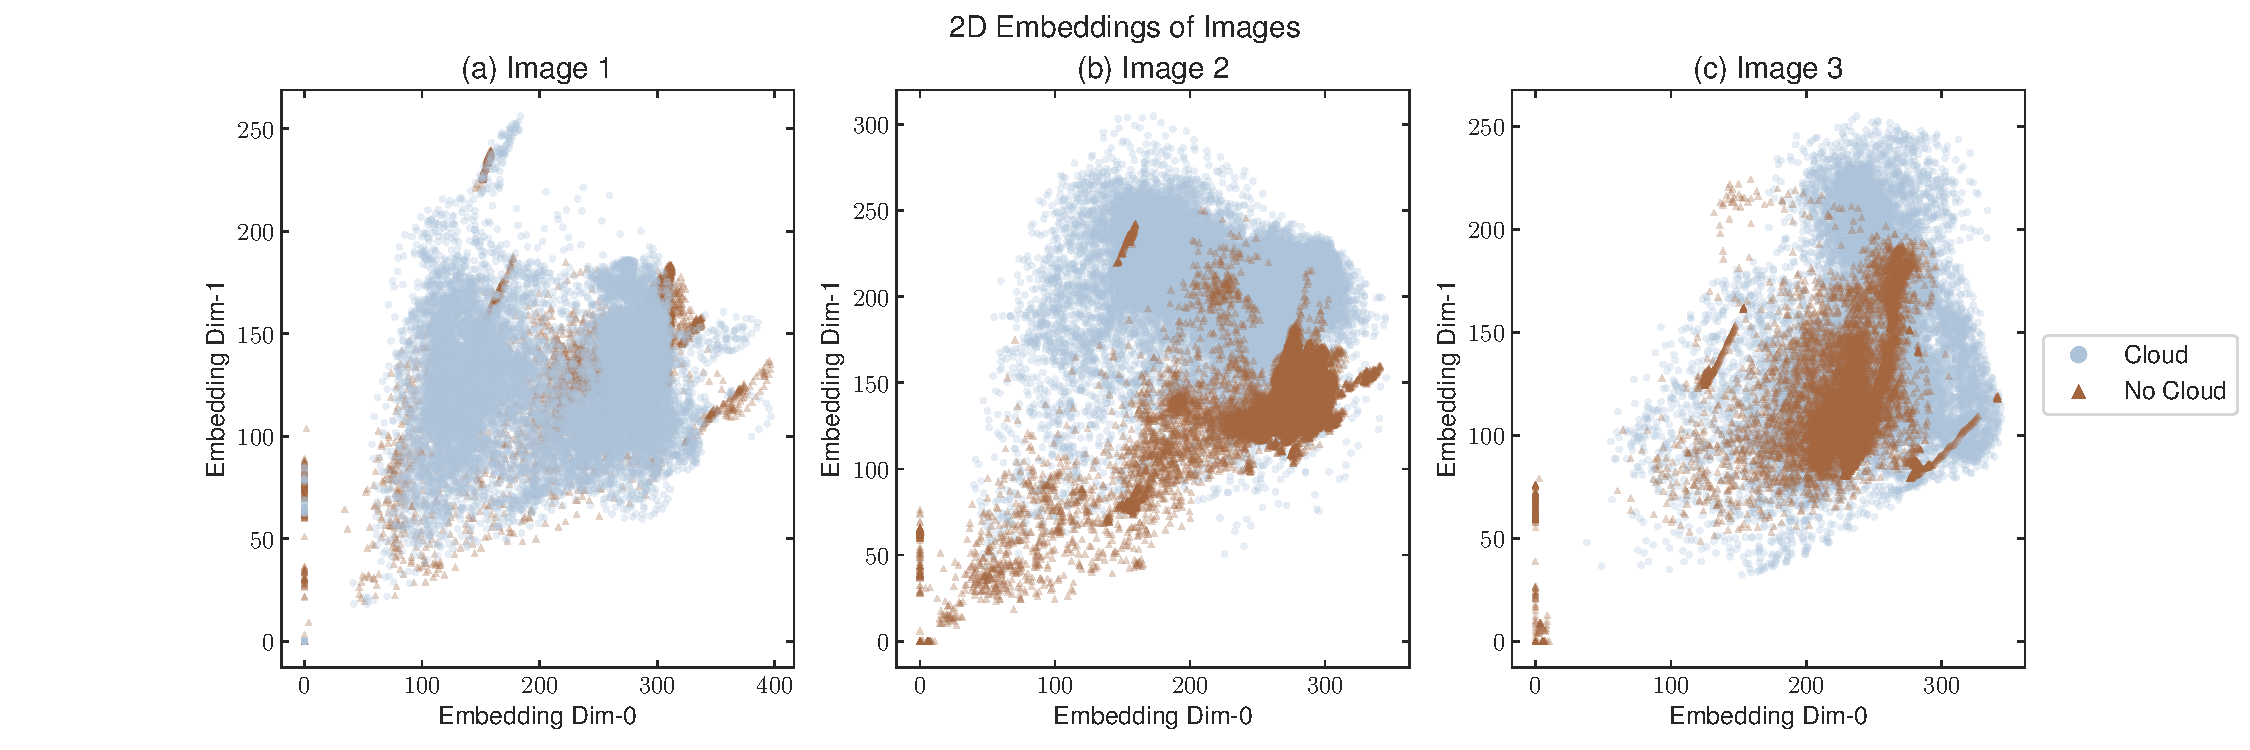
\includegraphics[width=\linewidth]{figs/embeddings.pdf}
    \caption{Scatter plot of embeddings generated by best auto-encoder model for cloud and non-cloud pixels.}
    \label{fig_embeddings}
\end{figure}

To further substantiate this observation, a correlation analysis is performed on the latent embeddings. Figure \ref{fig_emb_correlations} shows that the first latent component has a correlation coefficient of -0.11 with the cloud presence label, while the second component has a correlation of 0.46. These values indicate a weaker relationship compared to the NDAI and CORR features, suggesting that the Auto-encoder's latent representations are less effective in distinguishing cloud from non-cloud pixels. These results imply that the latent features are probably less useful for a classifier than the domain-specific ones, therefore, they are not applied in the modeling section.

\begin{figure}[H]
    \centering
    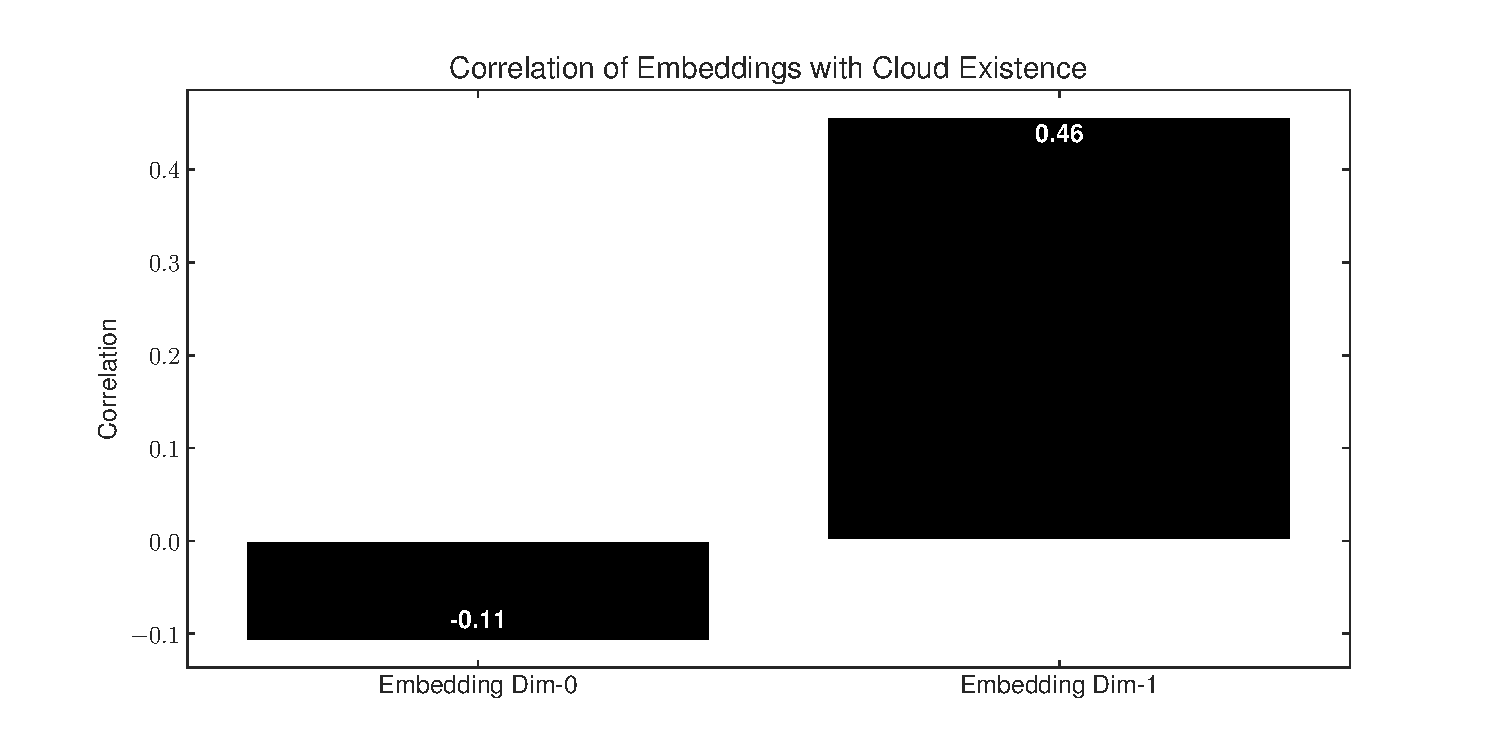
\includegraphics[width=\linewidth]{figs/correlation_embeddings.pdf}
    \caption{Point-biserial correlation coefficients of embedding components with cloud existence labels.}
    \label{fig_emb_correlations}
\end{figure}


\section{Data splitting}
To evaluate the generalizability of the models produced in this work, it is crucial to carefully split the data into training and testing sets. Given the spatial nature of the data, it is essential to ensure that the training and testing sets are spatially independent to prevent data leakage and overfitting. This means that the training and testing sets cannot simply be constructed by randomly sampling pixels from the images, as this would violate the spatial independence assumption. Instead, the data must be split by image. This work uses images 1 and 2 for training purposes and holds out image 3 for testing. This approach ensures that the models are evaluated on unseen data, providing a more accurate assessment of their performance on future observations.

During the modeling, the training data is further split into training and validation sets using two-fold cross-validation. This technique helps to tune the hyper-parameters of the models and assess their performance on different subsets of the training data. By using cross-validation, the models can be trained and evaluated multiple times, providing a more robust estimate of the optimal hyper-parameters. The final models are then trained on the full training data using the best hyper-parameters determined during cross-validation and evaluated on the held-out test data from image 3.

\section{Modeling}
This section outlines the different modeling approaches applied to the cloud detection task in the Arctic using radiance data from the MISR sensor aboard NASA's Terra satellite. More specifically, the assessed model architectures are logistic regression, random forest, weighted ensembles, and convolutional neural networks, providing a variety ranging from linear models through ensembles to deep neural networks. The subsequent sections provide a detailed analysis of each model, including their hyper-parameter tuning, performance metrics, and overall comparison on a held-out test set to determine which approach best fulfills the requirements for reliable cloud detection.

\subsection{Logistic Regression}
The first modeling algorithm that is applied to distinguish between cloud and non-cloud pixels in the Arctic using the radiance from the MISR sensor aboard NASA's Terra satellite is logistic regression through scikit-learn \parencite[]{scikit-learn}. The primary goal is to predict whether a given pixel represents a cloud (1.0) or non-cloud (-1.0) based on features derived from the sensor's multi-angle observations.

Hyper-parameter tuning is performed using two-fold cross-validation on the image 1 and image 2 datasets, searching for the optimal combination of regularization strength (C), penalty type, and ratio between L1 and L2 regularization if the chosen penalty is elastic net.
Table \ref{table:log_reg_hp_space} presents the hyper-parameter search space.

\begin{table}[]
\centering
\begin{tabular}{|l|l|}
\hline
\textbf{Hyper-parameter} & \textbf{Values} \\ \hline
Regularization Strength (C)                    & 0.01, 0.1, 1, 10, 100       \\
Penalty           & L1, L2, Elasticnet         \\
L1 ratio (only for Elasticnet)        & 0, 0.5, 1     \\ \hline
\end{tabular}
\caption{Hyper-parameter search space for Logistic Regression.}
\label{table:log_reg_hp_space}
\end{table}

The models are fitted on two different feature sets. The first feature set is the full feature set, which includes the raw angle features as well as the expert-derived features NDAI, CORR, and SD. The second feature set is reduced, as suggested by Sections \ref{sec:Data} and \ref{sec:feature_selection}, and contains only the expert-derived features NDAI, CORR, and SD. Table \ref{table:log_reg_best_hp} shows the best hyper-parameters for both feature sets. Interestingly, the best hyper-parameters are the same for both: L2 regularization and a C-value of 0.01.

\begin{table}[]
\centering
\begin{tabular}{|l|l|l|}
\hline
\textbf{Hyper-parameter}     & \textbf{Full Model} & \textbf{Reduced Model} \\ \hline
Regularization Strength (C) & L2                  & L2                     \\
Penalty                     & 0.01                & 0.01                   \\
L1 ratio                    & n/a                 & n/a                    \\ \hline
\end{tabular}
\caption{Best hyper-parameters for Logistic Regression.}
\label{table:log_reg_best_hp}
\end{table}

While the full model achieves a validation AUC score of 0.8267, the reduced model achieves a validation AUC score of 0.8965. Figure \ref{fig_roc_loc_regr} shows the ROC curves of both models on the test set (image 3). The curves are very similar, which is reflected by similar AUC scores on the test set: 0.89 for the full model and 0.9 for the reduced model. With a slightly higher AUC score, the reduced model achieves, on average, a higher true positive rate given a fixed false positive rate.

\begin{figure}[H]
    \centering
    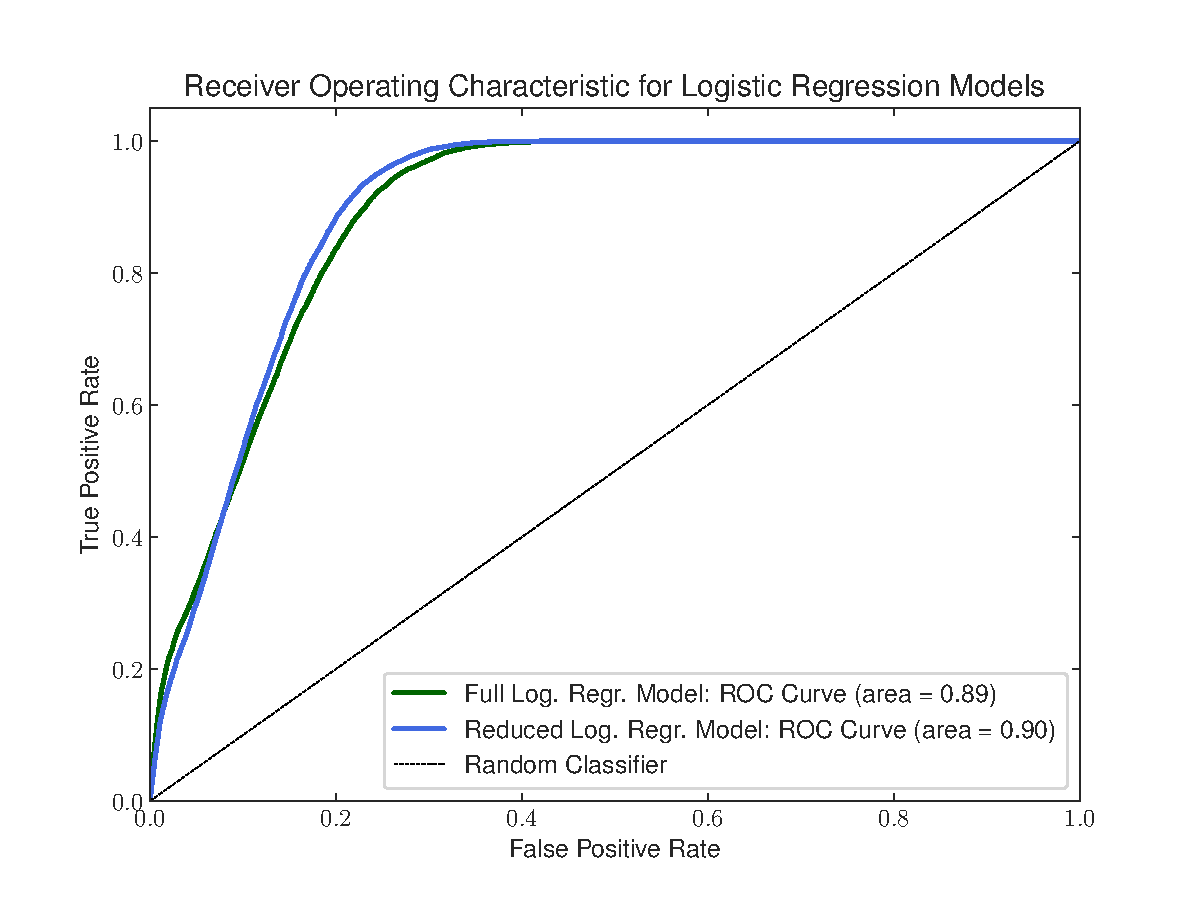
\includegraphics[width=\linewidth]{figs/roc_log_regr.pdf}
    \caption{Receiver Operating Characteristic curve for Logistic Regression models.}
    \label{fig_roc_loc_regr}
\end{figure}

\subsection{Random Forest}
Following logistic regression, random forest models were developed to apply non-linear modeling algorithms to the cloud detection data. Analogous to the previous section, two different models were developed using scikit-learn: (1) a full model using the features NDAI, SD, CORR, and the radiance angles DF, CF, BF, AF, and AN, and (2) a reduced model consisting of only NDAI, SD, and CORR after feature selection as suggested in Sections \ref{sec:Data} and \ref{sec:feature_selection} \parencite[]{scikit-learn}.

To tune the hyper-parameters of the random forests, two-fold cross-validation using image 1 and image was performed. Table \ref{table:random_forest_hp_space} shows the full hyper-parameter search space for both the full and the reduced model. Hyper-parameter tuning was conducted on the SCF Cluster, with a fixed random state to ensure reproducibility. The optimal set of hyper-parameters was identified through grid search, using the ROC AUC metric as the selection criterion. The best set of hyper-parameters is reported in Table \ref{table:best_hp_random_forest}. For the full model, they result in a validation AUC score of 0.9434, whereas the reduced model achieves a validation AUC score of 0.96.

\begin{table}[]
\centering
\begin{tabular}{|l|l|}
\hline
\textbf{Hyper-parameter} & \textbf{Values}  \\ \hline
Nr. of Estimators       & 100, 200, 300    \\
Max. depth              & None, 10, 20, 30 \\
Min. samples / split    & 2, 5, 10         \\
Min. samples / leaf     & 1, 2, 4          \\
Split Criterion         & Gini, Entropy    \\
Bootstrap               & True, False      \\ \hline
\end{tabular}
\caption{Hyper-parameter search space for Random Forest models.}
\label{table:random_forest_hp_space}
\end{table}

\begin{table}[]
\centering
\begin{tabular}{|l|l|l|}
\hline
\textbf{Hyper-parameter} & \textbf{Full Model} & \textbf{Reduced Model} \\ \hline
Nr. of Estimators        & 200                 & 100                    \\
Max. depth               & 10                  & 10                     \\
Min. samples / split     & 2                   & 10                     \\
Min. samples / leaf      & 4                   & 1                      \\
Split Criterion          & Entropy             & Gini                   \\
Bootstrap                & True                & False                  \\ \hline
\end{tabular}
\caption{Best hyper-parameters for the full and reduced Random Forest models.}
\label{table:best_hp_random_forest}
\end{table}

Using the best set of hyper-parameters from Table \ref{table:best_hp_random_forest}, both the full model and the reduced model fit on the combined data from image 1 and image 2. The full model shows a training accuracy of 96.79\%, while the prediction accuracy on the test data is significantly lower with only 47.6\%. This discrepancy between training accuracy and test accuracy might indicate overfitting issues. The reduced model does not have that high of a discrepancy, with a training accuracy of 95.64\% and a test accuracy of 81.30\%. This suggests that the reduced model has much better generalization capabilities.

Figure \ref{fig_rf_feature_importance} shows the impurity-based importance of the full model. Impurity-based feature importance measures the contribution of each feature to the reduction of impurity in the model while constructing the decision trees. Again, it can be observed that NDAI, CORR, and SD are the most significant features for the task of cloud detection, validating the feature selection in Sections \ref{sec:Data} and \ref{sec:feature_selection}.

\begin{figure}[H]
    \centering
    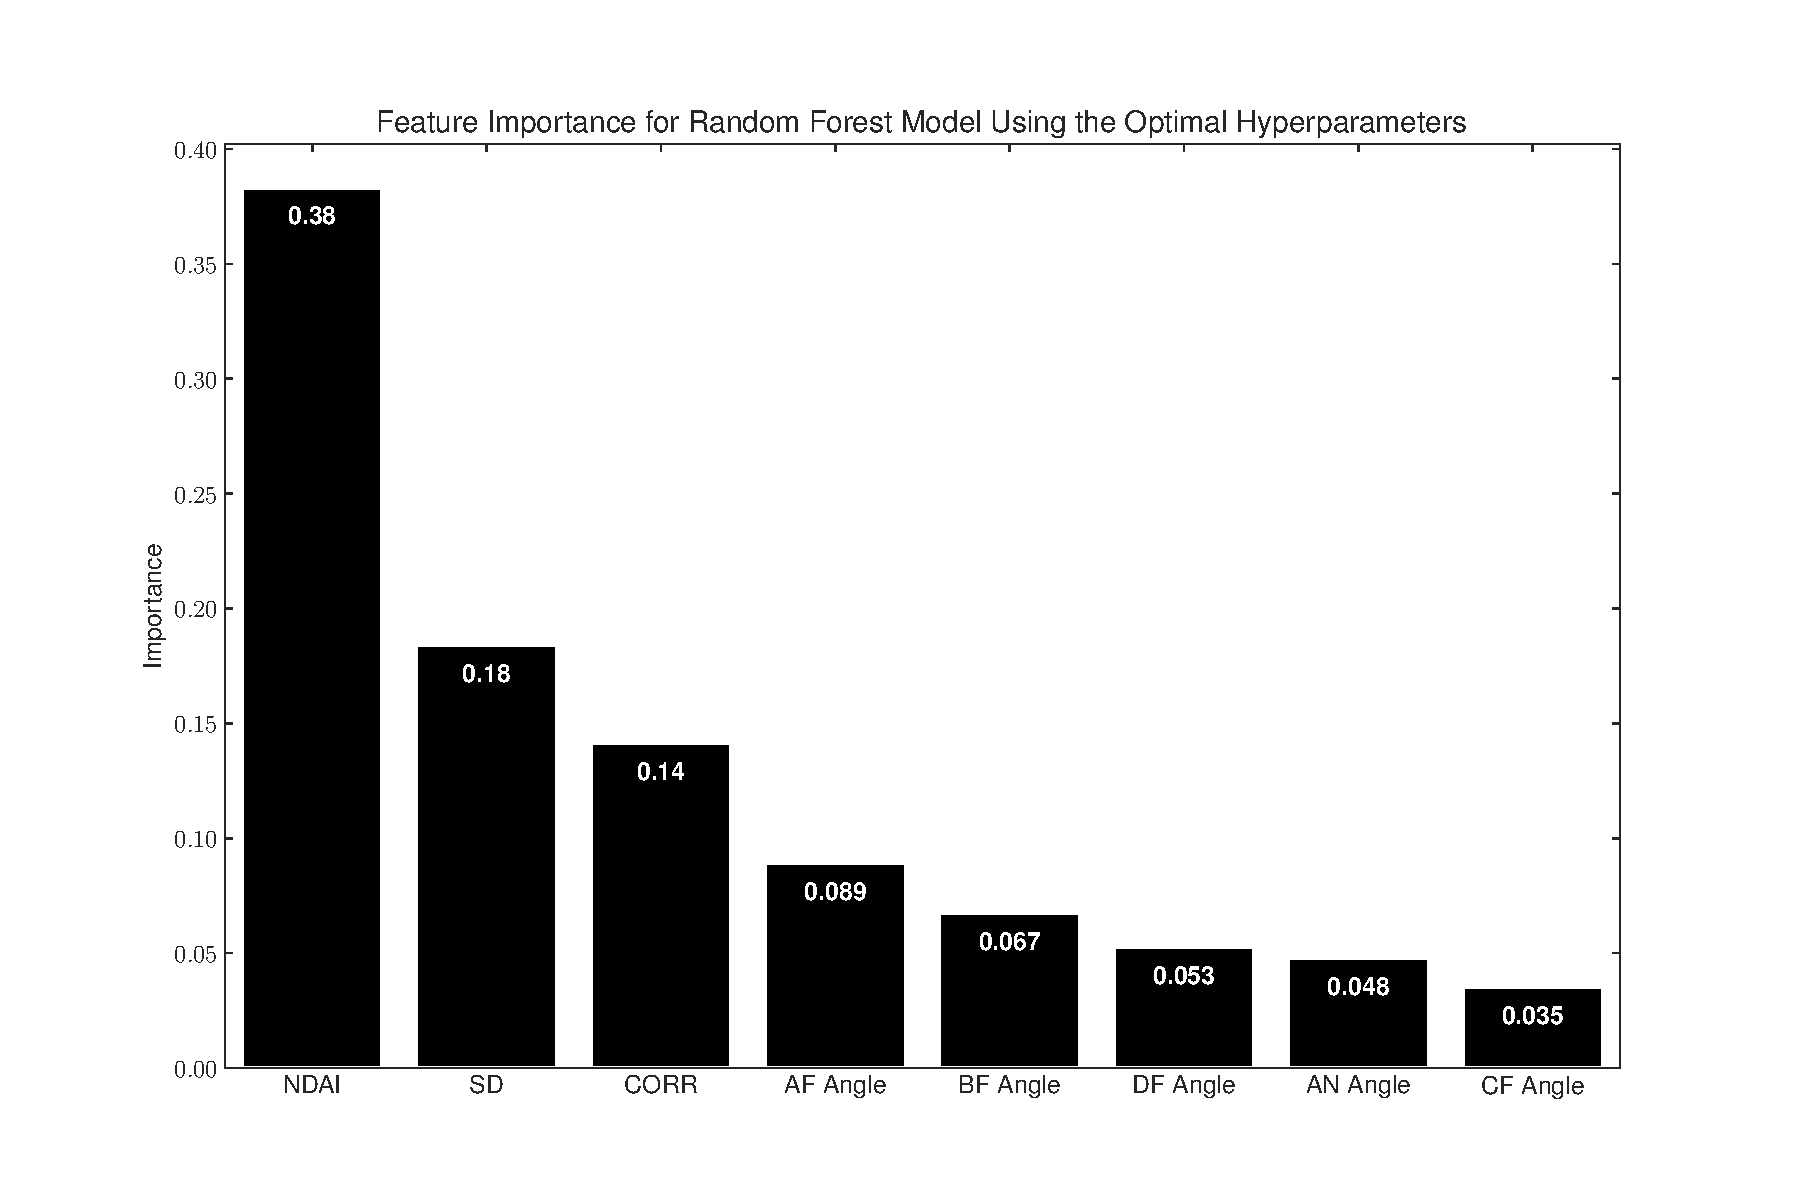
\includegraphics[width=0.9\linewidth]{figs/random_forest_feature_importance.pdf}
    \caption{Impurity-based feature importance for the full Random Forest model trained with optimal hyper-parameters.}
    \label{fig_rf_feature_importance}
\end{figure}

To better compare the performance of the full model to the reduced model, Figure \ref{fig_roc_random_forest} shows the ROC curve for both models on the test set (image 3). It is clearly visible that for all distinct false positive rates, the reduced model has a much higher true positive rate. This is also reflected by the much higher AUC score, which for the full model is only 0.62, whereas the reduced model achieves an AUC score of 0.9. This further demonstrates the superior generalization capabilities of the reduced model.

\begin{figure}[H]
    \centering
    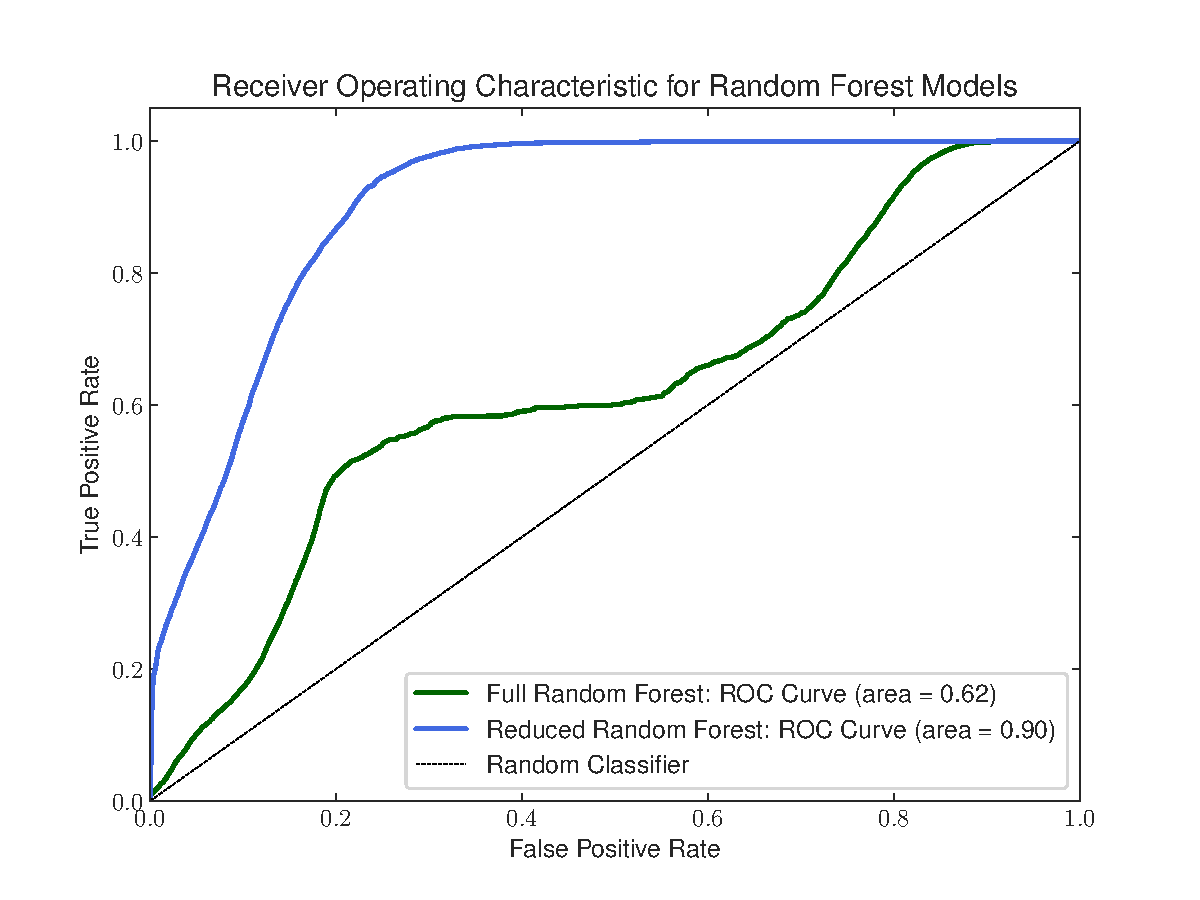
\includegraphics[width=0.9\linewidth]{figs/roc_random_forest.pdf}
    \caption{Receiver Operating Characteristic curve for Random Forest models..}
    \label{fig_roc_random_forest}
\end{figure}


\subsection{Weighted Ensemble}
This section describes modeling using AutoGluon, an automated machine-learning framework that enables rapid prototyping and evaluation of ensemble models. AutoGluon's approach to improving predictive performance involves a combination of bagging, cross-validation, and stacked ensembling. Unlike traditional methods that rely heavily on hyper-parameter tuning, AutoGluon focuses on assembling a diverse set of models to maximize stability and accuracy \parencite{autogluon}. This approach resembles random forests in that it ensembles multiple models. However, unlike random forests, it incorporates diverse model architectures and assigns different weights to the models based on their performance instead of weighing all models equally.

Bagging, or bootstrap aggregating, improves model robustness by training on different bootstrapped samples of the training data. This technique helps reduce overfitting and variance by averaging the predictions of multiple models. Stacked ensembling, on the other hand, combines multiple layers of models. The first layer consists of diverse base models trained on different subsets of the data, while the subsequent layers aggregate the predictions of the base models to make the final prediction. At the final layer, a meta-model is trained to learn the optimal combination of all previous predictions. This approach is also called weighted ensembling, as the meta-model assigns different weights to the predictions of the base models based on their performance.

Two different models were trained using AutoGluon: a full model utilizing all available features and a reduced model incorporating only NDAI, SD, and CORR, as identified through the feature selection analysis presented in Sections \ref{sec:Data} and \ref{sec:feature_selection}. For the full feature set, the best-performing ensemble model consisted of 26 models organized across three layers, while for the reduced feature set, the optimal model was notably more compact, comprising just five models split across two layers.

The best models were selected based on the highest area under the ROC curve (AUC) achieved during cross-validation between image 1 and image 2 data. Figure \ref{fig_roc_ensemble} illustrates the ROC curves for both the best-performing full and reduced models when evaluated on the test set (image 3). Notably, the full model achieved an AUC of 0.87, while the reduced model performed better with an AUC of 0.92, representing a five percentage point improvement.

From the ROC curves in Figure \ref{fig_roc_ensemble}, it is evident that the reduced model consistently outperforms the full model across different thresholds. Only for very low false positive rates the full model achieves a slightly higher true positive rate. Specifically, for thresholds resulting in a false positive rate below 0.3, the reduced model demonstrates a higher true positive rate. This suggests that the reduced model is more effective at detecting clouds while minimizing false positives, making it a more reliable option.

\begin{figure}[H]
    \centering
    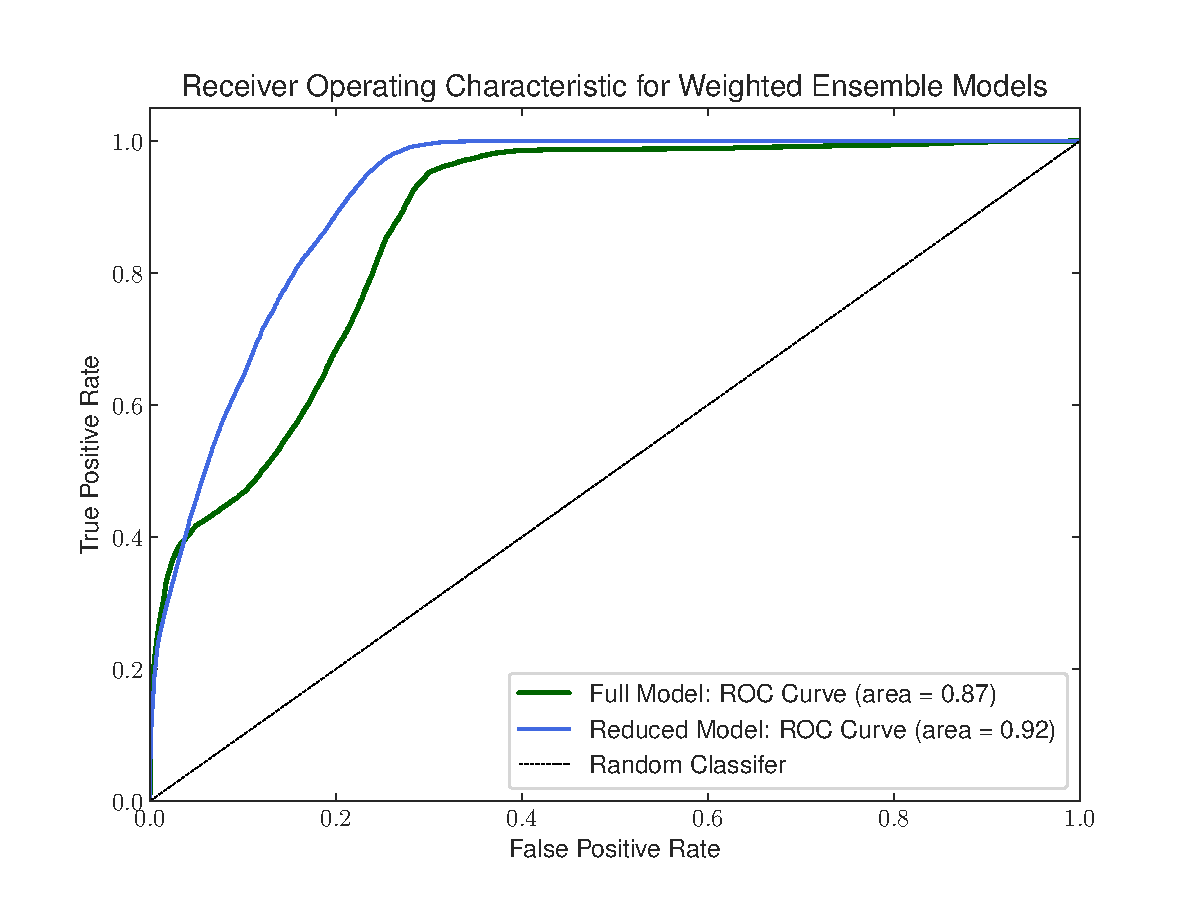
\includegraphics[width=0.9\linewidth]{figs/roc_ensemble.pdf}
    \caption{Receiver Operating Characteristic curve for Weighted Ensemble Models.}
    \label{fig_roc_ensemble}
\end{figure}

\subsection{Convolutional Neural Network}
Given that the data is image-like, a Convolutional Neural Network (CNN) is a natural choice for modeling the cloud detection problem. CNNs make the location invariance assumption, meaning that they can learn spatial patterns in the data regardless of their location in the image. This property makes CNNs well-suited for image classification tasks. In this work, the U-Net architecture is adapted, as it shows promising results in image segmentation tasks in the biomedical domain \parencite[]{unet}.

The U-Net architecture consists of an encoder-decoder structure with skip connections that help preserve spatial information during the downsampling and upsampling operations. The encoder is composed of convolutional and pooling layers that gradually reduce the spatial dimensions of the input data, while the decoder consists of upsampling and convolutional layers that gradually increase the spatial dimensions back to the original input size. Skip connections link the encoder and decoder at corresponding spatial resolutions, enabling the model to combine both low-level and high-level features during the upsampling process. This allows the model to provide classification predictions at the pixel level.

Similar to the process of training the auto-encoder as described in Section \ref{sec:feature_selection}, the U-Net segmentation model is trained using PyTorch Lightning \parencite[]{pytorch_lightning}. The hyper-parameters of the U-Net model are tuned using image 1 as the training data and image 2 as the validation data using Weights \& Biases' sweep functionality \parencite{wandb}. Table \ref{table:cnn_hp_space} shows the search space for the hyper-parameters, which includes the set of features to use and whether to apply image augmentation. Given the scarcity of training data, image augmentation is applied to artificially increase the size of the training set. The augmentation techniques include random flips and rotations, as these operations do not alter the values of the features but simply provide a different perspective of the image. The loss function used is binary cross-entropy, with unlabeled pixels being ignored for the loss calculation.

\begin{table}[]
\centering
\begin{tabular}{|l|l|}
\hline
\textbf{Hyper-parameter} & \textbf{Values}                      \\ \hline
Feature Set             & All, Angle-only, Expert-features-only \\
Image Augmentation      & True, False                           \\ \hline
\end{tabular}
\caption{Hyper-parameter search space for the CNN classifier.}
\label{table:cnn_hp_space}
\end{table}

Since the AUC metric is found to be unstable when using a single training sample, the best model is selected based on the highest accuracy on the validation set. Similar to the approach used with the Auto-encoder, early stopping is employed to prevent overfitting and reduce training time. The models are trained for a maximum of 100 epochs, with a patience of 10 epochs before early stopping is applied. The best hyper-parameters are shown in Table \ref{table:cnn_best_hp}, which result in a validation accuracy of 0.9591. The best result is achieved when using only the raw angles as features and not applying image augmentation. This suggests that the model is capable of learning meaningful features from the raw data without relying on expert-derived features.

\begin{table}[]
\centering
\begin{tabular}{|l|l|}
\hline
\textbf{Hyper-parameter} & \textbf{Value}                    \\ \hline
Feature Set             & Angle-only                         \\
Image Augmentation      & False                              \\ \hline
\end{tabular}
\caption{Best hyper-parameters for CNN classifier.}
\label{table:cnn_best_hp}
\end{table}

The best model is then evaluated on the test data from image 3 to assess its generalization performance. Figure \ref{fig_roc_cnn} shows the ROC curve, with an AUC of only 0.79, indicating that the model does not generalize as well to the test data as the models from previous sections. One possible reason for this is the small size of the training dataset. Deep learning models typically require large amounts of data to generalize well to unseen observations, and the limited training data in this work might not be sufficient to fit the complex U-Net architecture effectively.

\begin{figure}[H]
    \centering
    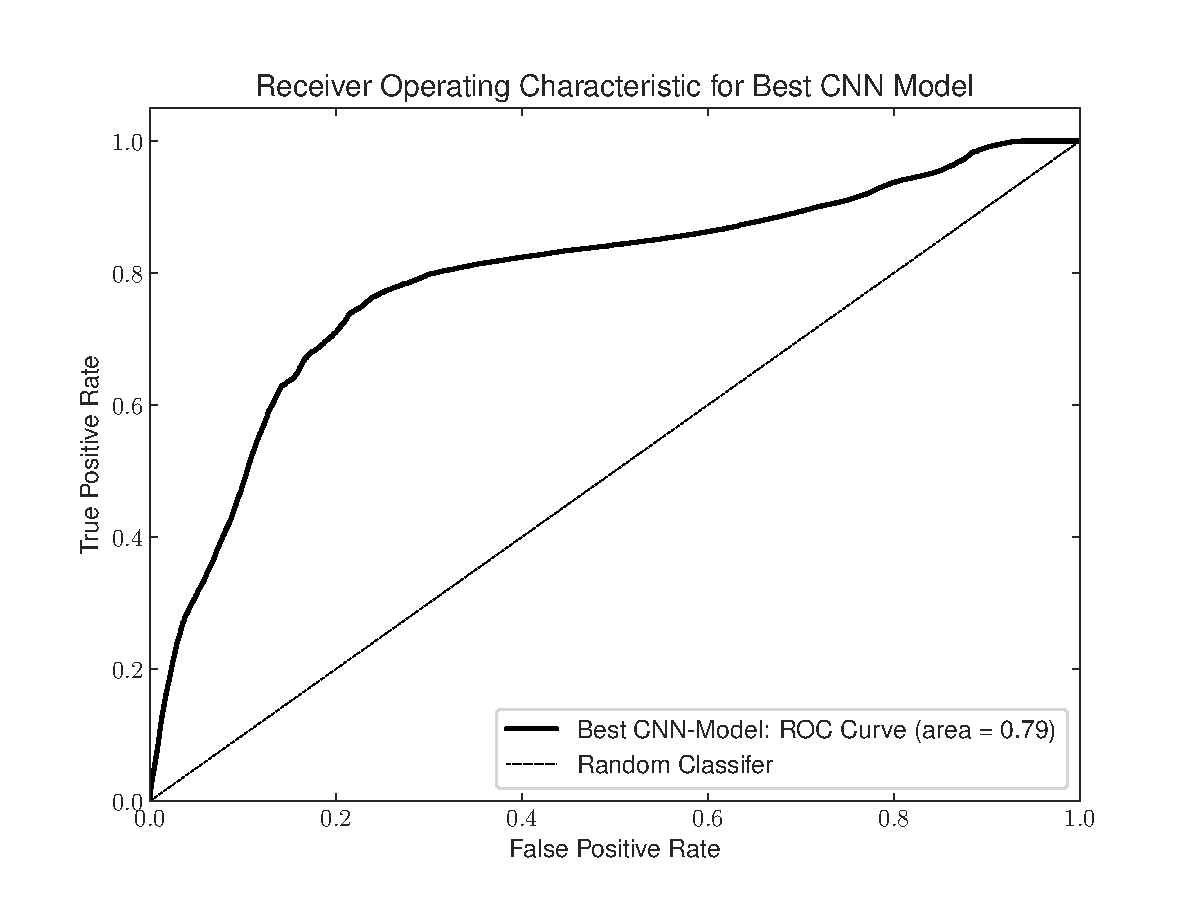
\includegraphics[width=0.9\linewidth]{figs/roc_cnn.pdf}
    \caption{Receiver Operating Characteristic curve for best CNN classifier.}
    \label{fig_roc_cnn}
\end{figure}


\subsection{Model Comparison}
Given the large number of models developed throughout this report, it is important to compare them on an unseen test set to determine which one best fulfills the need for reliably performing cloud detection. Figure \ref{fig_roc_all} shows the ROC curve for the best models from each approach presented: logistic regression, random forest, weighted ensemble, and a convolutional neural network (CNN). It is interesting to note that for all approaches, the best model is one based on a reduced feature set rather than using all available features. The models are compared based on AUC scores due to the fact that the AUC score is threshold agnostic. This provides an evaluation of model performance across all possible classification thresholds.

\begin{figure}[H]
    \centering
    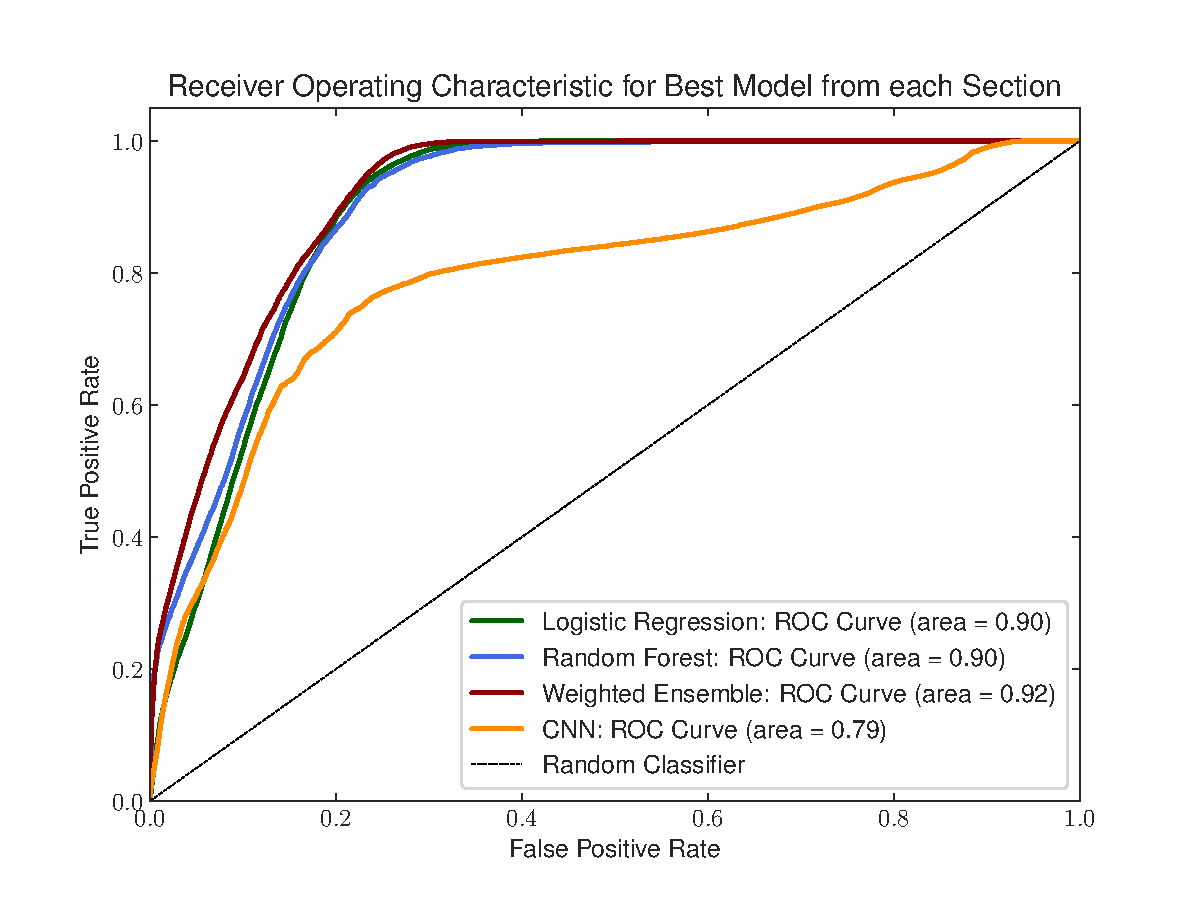
\includegraphics[width=0.9\linewidth]{figs/roc_all_models.pdf}
    \caption{Receiver Operating Characteristic curve for the best model from each section.}
    \label{fig_roc_all}
\end{figure}

From the ROC curves, it is evident that the CNN demonstrates significantly lower performance compared to the other models, with an AUC score of 0.79. The underperformance of the CNN could be attributed to the limited training data, which might be insufficient for the complexity of the CNN architecture to generalize effectively.

The other models show a similar performance, achieving AUC scores around 0.9. The best model is the weighted ensemble model, which reaches an AUC score of 0.92 on unseen test data. Given that the weighted ensemble performs best with regard to AUC scores, the remainder of this report focuses on analyzing where this model has difficulties in making precise predictions.

\subsection{Stability Analysis}
This section explores the stability of the weighted ensemble model with respect to different train-test splits. The original reduced weighted ensemble model used image 1 and image 2 as the training set and was evaluated on image 3. To assess the model's stability, this process was repeated with different train-test splits: one split used image 1 as the test set and images 2 and 3 as the training set, while another used image 2 as the test set and images 1 and 3 for training.

Figure \ref{fig_roc_stability} shows the ROC curves of the three different models. It can be concluded that the train-test split does not significantly influence the model's performance. All three models achieve similar AUC scores between 0.92 and 0.98. Additionally, the ROC curves for all three models follow a nearly identical path. This provides evidence that the performance of the reduced weighted ensemble model is stable across different train-test splits.

\begin{figure}[H]
    \centering
    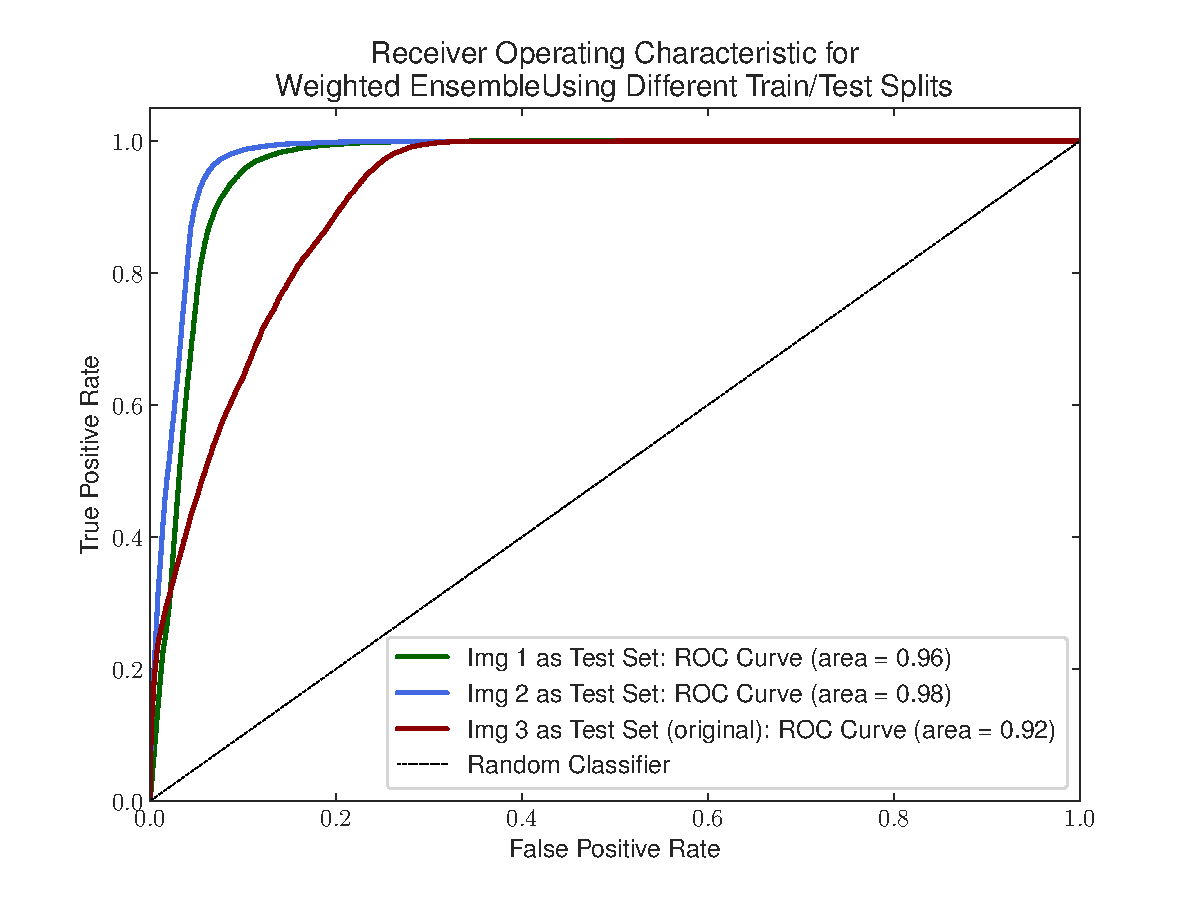
\includegraphics[width=\linewidth]{figs/roc_stability.pdf}
    \caption{Receiver Operating Characteristic curves for reduced weighted ensemble models trained and evaluated on different train/test splits.}
    \label{fig_roc_stability}
\end{figure}

\subsection{Error Analysis}
This section focuses on determining the shortcomings of the best-performing model, the weights ensemble model fit on the reduced feature set. Figure \ref{fig_classification_metrics} shows common performance metrics for binary classification tasks, determined on the test set (image 3). It is important to note that these metrics are calculated using a decision threshold of 0.5. The decision threshold could be adapted to optimize the model's performance for a specific metric, however, this would require another tuning dataset, which is not available due to the limited data available for this report.

\begin{figure}[H]
    \centering
    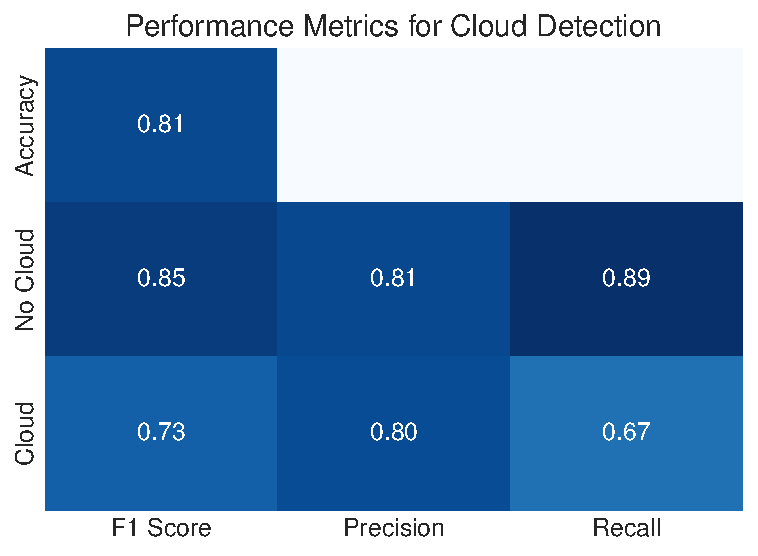
\includegraphics[width=0.9\linewidth]{figs/post_hoc_eda.pdf}
    \caption{Precision, Recall, F1-Score, and Accuracy for the reduced weighted ensemble model on the "Cloud" and "No Cloud" label determined based on the test set (image 3).}
    \label{fig_classification_metrics}
\end{figure}

The precision is similar for both the "Cloud" and "No Cloud" classes. The recall for the "No Cloud" label, however, is notably higher by 22 percentage points. This indicates that the model has a bias towards classifying pixels as "No Cloud" rather than "Cloud". One possible reason for this bias could be the slight label imbalance observed in the dataset. As shown in Figure \ref{fig_eda_label_distrib} in Section \ref{sec:Data}, there is a difference of more than 12 percentage points between the number of data points labeled as "No Cloud" and "Cloud". The model's overall accuracy is 81\%, which means that the majority of the predictions are correct, but there are still notable areas for improvement.

Figure \ref{fig_error_analysis} provides an understanding of the areas where the model makes mistakes. It can be observed that most errors occur in cloud regions that are misclassified as "No Cloud". This explains the lower recall values for the "Cloud" label. Furthermore, it can be concluded that the model is more confident in its predictions in areas where the ground truth label is "No Cloud".

\begin{figure}[H]
    \centering
    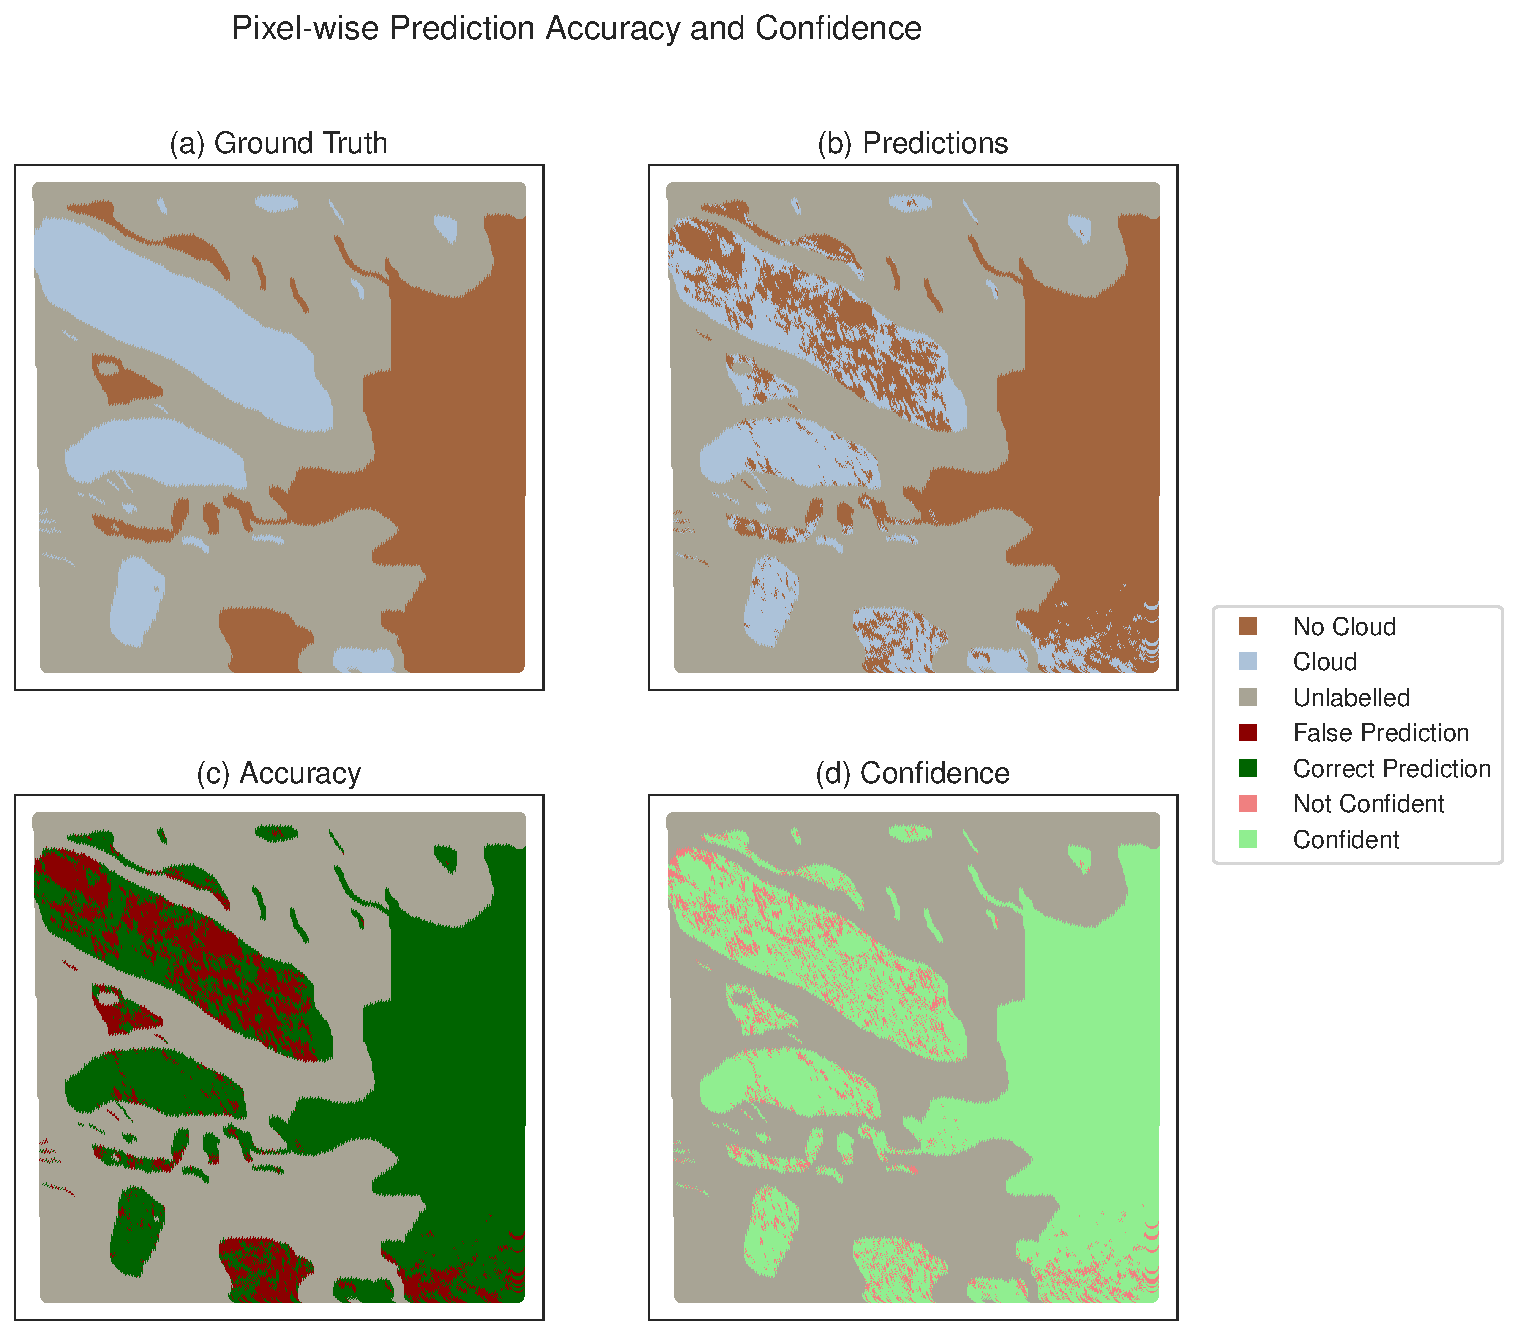
\includegraphics[width=\linewidth]{figs/error_analysis.pdf}
    \caption{Pixel-wise predictions, accuracy, and confidence of the reduced weighted ensemble model on the test set (image 3). The model is defined to be confident if the predicted probability for the "Cloud" class is less than 0.4 or greater than 0.6.}
    \label{fig_error_analysis}
\end{figure}

To improve the model, future efforts could focus on refining the decision threshold or incorporating additional contextual features that may help the model better differentiate between cloud and non-cloud regions.

\section{Conclusion}
This report aimed to develop an effective approach for detecting clouds in the Arctic using radiance data from the MISR sensor aboard NASA's Terra satellite. Several modeling techniques were explored, including logistic regression, random forest, weighted ensembles, and convolutional neural networks (CNNs). The models were evaluated in terms of their ability to distinguish between cloud and non-cloud pixels using both full and reduced feature sets.

Through the analysis, it became evident that the reduced feature set, which consisted of NDAI, SD, and CORR, outperformed the full feature set across all approaches, except for the CNN, which achieved the highest validation accuracy using only the raw features. The weighted ensemble model provided the best overall performance, achieving an AUC score of 0.92 on the test data, highlighting its ability to generalize well to unseen observations. The random forest and logistic regression models also performed comparably well, while the CNN struggled to reach similar performance levels, likely due to limited training data.

The error analysis showed that the model faced challenges in misclassifying cloud areas as non-cloud, with a bias toward predicting non-cloud pixels over cloud pixels. This bias could be attributed to label imbalance and the inherent difficulty in distinguishing cloud features from other reflective surfaces in the Arctic. Addressing this limitation is crucial for future improvements, which could be as simple as refining the decision threshold or more complex such as incorporating additional contextual information to better separate cloud and non-cloud regions.

Future work may, additionally, focus on further refining the features, balancing the dataset, exploring additional data sources, and conducting a more extensive hyper-parameter search to enhance model robustness and accuracy in challenging conditions. For example, many of the hyper-parameters for the CNN, like the learning rate, were set to default values, and optimizing these could lead to better performance. Future work on CNNs could, furthermore, focus on training deep neural networks with larger datasets to enhance their generalization capabilities. One of the primary strengths of deep learning is its ability to automatically learn features from raw input data, reducing the need for manual feature engineering.

The research conducted in this report is important for predicting the development of climate-related patterns in the Arctic. Understanding cloud behavior can help improve climate models, contributing to better-informed decisions that may help to decelerate climate change.

\newpage
\printbibliography

\appendix
\section{Academic honesty}
\subsection{Statement}
Hereby, we confirm that this report is the result of our own work and that any ideas and findings from others, including our classmates, have been properly cited and referenced. Academic research honesty is essential to ensure trust in the scientific community. Research is a collaborative effort that relies on constantly building upon the work of others. It is, therefore, crucial to provide the sources of information used in scientific work in order for the research community to verify, reproduce, and build upon the findings.
\subsection{Collaborators}
There are no other collaborators outside our group.
\subsection{LLM Usage}

\subsubsection*{Coding}
For coding, we used co-pilot to help us write some code and debug. We tried to write most comments, but some comments were made by tab-completing individual lines. Overall, using co-pilot is a good experience for simple algorithms. It also helps us make better graphs. It's very convenient, but sometimes it's not reliable. It's important to understand and check the code thoroughly because co-pilot can make some mistakes. We would use co-pilot again for similar projects.

\subsubsection*{Writing}
For writing, we wrote everything on our own and then used LLM (Grammarly) to check basic grammar and spelling errors.

\end{document}
